\documentclass[11pt]{article}

    \usepackage[breakable]{tcolorbox}
    \usepackage{parskip} % Stop auto-indenting (to mimic markdown behaviour)
    

    % Basic figure setup, for now with no caption control since it's done
    % automatically by Pandoc (which extracts ![](path) syntax from Markdown).
    \usepackage{graphicx}
    % Maintain compatibility with old templates. Remove in nbconvert 6.0
    \let\Oldincludegraphics\includegraphics
    % Ensure that by default, figures have no caption (until we provide a
    % proper Figure object with a Caption API and a way to capture that
    % in the conversion process - todo).
    \usepackage{caption}
    \DeclareCaptionFormat{nocaption}{}
    \captionsetup{format=nocaption,aboveskip=0pt,belowskip=0pt}

    \usepackage{float}
    \floatplacement{figure}{H} % forces figures to be placed at the correct location
    \usepackage{xcolor} % Allow colors to be defined
    \usepackage{enumerate} % Needed for markdown enumerations to work
    \usepackage{geometry} % Used to adjust the document margins
    \usepackage{amsmath} % Equations
    \usepackage{amssymb} % Equations
    \usepackage{textcomp} % defines textquotesingle
    % Hack from http://tex.stackexchange.com/a/47451/13684:
    \AtBeginDocument{%
        \def\PYZsq{\textquotesingle}% Upright quotes in Pygmentized code
    }
    \usepackage{upquote} % Upright quotes for verbatim code
    \usepackage{eurosym} % defines \euro

    \usepackage{iftex}
    \ifPDFTeX
        \usepackage[T1]{fontenc}
        \IfFileExists{alphabeta.sty}{
              \usepackage{alphabeta}
          }{
              \usepackage[mathletters]{ucs}
              \usepackage[utf8x]{inputenc}
          }
    \else
        \usepackage{fontspec}
        \usepackage{unicode-math}
    \fi

    \usepackage{fancyvrb} % verbatim replacement that allows latex
    \usepackage{grffile} % extends the file name processing of package graphics
                         % to support a larger range
    \makeatletter % fix for old versions of grffile with XeLaTeX
    \@ifpackagelater{grffile}{2019/11/01}
    {
      % Do nothing on new versions
    }
    {
      \def\Gread@@xetex#1{%
        \IfFileExists{"\Gin@base".bb}%
        {\Gread@eps{\Gin@base.bb}}%
        {\Gread@@xetex@aux#1}%
      }
    }
    \makeatother
    \usepackage[Export]{adjustbox} % Used to constrain images to a maximum size
    \adjustboxset{max size={0.9\linewidth}{0.9\paperheight}}

    % The hyperref package gives us a pdf with properly built
    % internal navigation ('pdf bookmarks' for the table of contents,
    % internal cross-reference links, web links for URLs, etc.)
    \usepackage{hyperref}
    % The default LaTeX title has an obnoxious amount of whitespace. By default,
    % titling removes some of it. It also provides customization options.
    \usepackage{titling}
    \usepackage{longtable} % longtable support required by pandoc >1.10
    \usepackage{booktabs}  % table support for pandoc > 1.12.2
    \usepackage{array}     % table support for pandoc >= 2.11.3
    \usepackage{calc}      % table minipage width calculation for pandoc >= 2.11.1
    \usepackage[inline]{enumitem} % IRkernel/repr support (it uses the enumerate* environment)
    \usepackage[normalem]{ulem} % ulem is needed to support strikethroughs (\sout)
                                % normalem makes italics be italics, not underlines
    \usepackage{mathrsfs}
    

    
    % Colors for the hyperref package
    \definecolor{urlcolor}{rgb}{0,.145,.698}
    \definecolor{linkcolor}{rgb}{.71,0.21,0.01}
    \definecolor{citecolor}{rgb}{.12,.54,.11}

    % ANSI colors
    \definecolor{ansi-black}{HTML}{3E424D}
    \definecolor{ansi-black-intense}{HTML}{282C36}
    \definecolor{ansi-red}{HTML}{E75C58}
    \definecolor{ansi-red-intense}{HTML}{B22B31}
    \definecolor{ansi-green}{HTML}{00A250}
    \definecolor{ansi-green-intense}{HTML}{007427}
    \definecolor{ansi-yellow}{HTML}{DDB62B}
    \definecolor{ansi-yellow-intense}{HTML}{B27D12}
    \definecolor{ansi-blue}{HTML}{208FFB}
    \definecolor{ansi-blue-intense}{HTML}{0065CA}
    \definecolor{ansi-magenta}{HTML}{D160C4}
    \definecolor{ansi-magenta-intense}{HTML}{A03196}
    \definecolor{ansi-cyan}{HTML}{60C6C8}
    \definecolor{ansi-cyan-intense}{HTML}{258F8F}
    \definecolor{ansi-white}{HTML}{C5C1B4}
    \definecolor{ansi-white-intense}{HTML}{A1A6B2}
    \definecolor{ansi-default-inverse-fg}{HTML}{FFFFFF}
    \definecolor{ansi-default-inverse-bg}{HTML}{000000}

    % common color for the border for error outputs.
    \definecolor{outerrorbackground}{HTML}{FFDFDF}

    % commands and environments needed by pandoc snippets
    % extracted from the output of `pandoc -s`
    \providecommand{\tightlist}{%
      \setlength{\itemsep}{0pt}\setlength{\parskip}{0pt}}
    \DefineVerbatimEnvironment{Highlighting}{Verbatim}{commandchars=\\\{\}}
    % Add ',fontsize=\small' for more characters per line
    \newenvironment{Shaded}{}{}
    \newcommand{\KeywordTok}[1]{\textcolor[rgb]{0.00,0.44,0.13}{\textbf{{#1}}}}
    \newcommand{\DataTypeTok}[1]{\textcolor[rgb]{0.56,0.13,0.00}{{#1}}}
    \newcommand{\DecValTok}[1]{\textcolor[rgb]{0.25,0.63,0.44}{{#1}}}
    \newcommand{\BaseNTok}[1]{\textcolor[rgb]{0.25,0.63,0.44}{{#1}}}
    \newcommand{\FloatTok}[1]{\textcolor[rgb]{0.25,0.63,0.44}{{#1}}}
    \newcommand{\CharTok}[1]{\textcolor[rgb]{0.25,0.44,0.63}{{#1}}}
    \newcommand{\StringTok}[1]{\textcolor[rgb]{0.25,0.44,0.63}{{#1}}}
    \newcommand{\CommentTok}[1]{\textcolor[rgb]{0.38,0.63,0.69}{\textit{{#1}}}}
    \newcommand{\OtherTok}[1]{\textcolor[rgb]{0.00,0.44,0.13}{{#1}}}
    \newcommand{\AlertTok}[1]{\textcolor[rgb]{1.00,0.00,0.00}{\textbf{{#1}}}}
    \newcommand{\FunctionTok}[1]{\textcolor[rgb]{0.02,0.16,0.49}{{#1}}}
    \newcommand{\RegionMarkerTok}[1]{{#1}}
    \newcommand{\ErrorTok}[1]{\textcolor[rgb]{1.00,0.00,0.00}{\textbf{{#1}}}}
    \newcommand{\NormalTok}[1]{{#1}}

    % Additional commands for more recent versions of Pandoc
    \newcommand{\ConstantTok}[1]{\textcolor[rgb]{0.53,0.00,0.00}{{#1}}}
    \newcommand{\SpecialCharTok}[1]{\textcolor[rgb]{0.25,0.44,0.63}{{#1}}}
    \newcommand{\VerbatimStringTok}[1]{\textcolor[rgb]{0.25,0.44,0.63}{{#1}}}
    \newcommand{\SpecialStringTok}[1]{\textcolor[rgb]{0.73,0.40,0.53}{{#1}}}
    \newcommand{\ImportTok}[1]{{#1}}
    \newcommand{\DocumentationTok}[1]{\textcolor[rgb]{0.73,0.13,0.13}{\textit{{#1}}}}
    \newcommand{\AnnotationTok}[1]{\textcolor[rgb]{0.38,0.63,0.69}{\textbf{\textit{{#1}}}}}
    \newcommand{\CommentVarTok}[1]{\textcolor[rgb]{0.38,0.63,0.69}{\textbf{\textit{{#1}}}}}
    \newcommand{\VariableTok}[1]{\textcolor[rgb]{0.10,0.09,0.49}{{#1}}}
    \newcommand{\ControlFlowTok}[1]{\textcolor[rgb]{0.00,0.44,0.13}{\textbf{{#1}}}}
    \newcommand{\OperatorTok}[1]{\textcolor[rgb]{0.40,0.40,0.40}{{#1}}}
    \newcommand{\BuiltInTok}[1]{{#1}}
    \newcommand{\ExtensionTok}[1]{{#1}}
    \newcommand{\PreprocessorTok}[1]{\textcolor[rgb]{0.74,0.48,0.00}{{#1}}}
    \newcommand{\AttributeTok}[1]{\textcolor[rgb]{0.49,0.56,0.16}{{#1}}}
    \newcommand{\InformationTok}[1]{\textcolor[rgb]{0.38,0.63,0.69}{\textbf{\textit{{#1}}}}}
    \newcommand{\WarningTok}[1]{\textcolor[rgb]{0.38,0.63,0.69}{\textbf{\textit{{#1}}}}}


    % Define a nice break command that doesn't care if a line doesn't already
    % exist.
    \def\br{\hspace*{\fill} \\* }
    % Math Jax compatibility definitions
    \def\gt{>}
    \def\lt{<}
    \let\Oldtex\TeX
    \let\Oldlatex\LaTeX
    \renewcommand{\TeX}{\textrm{\Oldtex}}
    \renewcommand{\LaTeX}{\textrm{\Oldlatex}}
    % Document parameters
    % Document title
    \title{SBJ\_example}
    
    
    
    
    
% Pygments definitions
\makeatletter
\def\PY@reset{\let\PY@it=\relax \let\PY@bf=\relax%
    \let\PY@ul=\relax \let\PY@tc=\relax%
    \let\PY@bc=\relax \let\PY@ff=\relax}
\def\PY@tok#1{\csname PY@tok@#1\endcsname}
\def\PY@toks#1+{\ifx\relax#1\empty\else%
    \PY@tok{#1}\expandafter\PY@toks\fi}
\def\PY@do#1{\PY@bc{\PY@tc{\PY@ul{%
    \PY@it{\PY@bf{\PY@ff{#1}}}}}}}
\def\PY#1#2{\PY@reset\PY@toks#1+\relax+\PY@do{#2}}

\@namedef{PY@tok@w}{\def\PY@tc##1{\textcolor[rgb]{0.73,0.73,0.73}{##1}}}
\@namedef{PY@tok@c}{\let\PY@it=\textit\def\PY@tc##1{\textcolor[rgb]{0.24,0.48,0.48}{##1}}}
\@namedef{PY@tok@cp}{\def\PY@tc##1{\textcolor[rgb]{0.61,0.40,0.00}{##1}}}
\@namedef{PY@tok@k}{\let\PY@bf=\textbf\def\PY@tc##1{\textcolor[rgb]{0.00,0.50,0.00}{##1}}}
\@namedef{PY@tok@kp}{\def\PY@tc##1{\textcolor[rgb]{0.00,0.50,0.00}{##1}}}
\@namedef{PY@tok@kt}{\def\PY@tc##1{\textcolor[rgb]{0.69,0.00,0.25}{##1}}}
\@namedef{PY@tok@o}{\def\PY@tc##1{\textcolor[rgb]{0.40,0.40,0.40}{##1}}}
\@namedef{PY@tok@ow}{\let\PY@bf=\textbf\def\PY@tc##1{\textcolor[rgb]{0.67,0.13,1.00}{##1}}}
\@namedef{PY@tok@nb}{\def\PY@tc##1{\textcolor[rgb]{0.00,0.50,0.00}{##1}}}
\@namedef{PY@tok@nf}{\def\PY@tc##1{\textcolor[rgb]{0.00,0.00,1.00}{##1}}}
\@namedef{PY@tok@nc}{\let\PY@bf=\textbf\def\PY@tc##1{\textcolor[rgb]{0.00,0.00,1.00}{##1}}}
\@namedef{PY@tok@nn}{\let\PY@bf=\textbf\def\PY@tc##1{\textcolor[rgb]{0.00,0.00,1.00}{##1}}}
\@namedef{PY@tok@ne}{\let\PY@bf=\textbf\def\PY@tc##1{\textcolor[rgb]{0.80,0.25,0.22}{##1}}}
\@namedef{PY@tok@nv}{\def\PY@tc##1{\textcolor[rgb]{0.10,0.09,0.49}{##1}}}
\@namedef{PY@tok@no}{\def\PY@tc##1{\textcolor[rgb]{0.53,0.00,0.00}{##1}}}
\@namedef{PY@tok@nl}{\def\PY@tc##1{\textcolor[rgb]{0.46,0.46,0.00}{##1}}}
\@namedef{PY@tok@ni}{\let\PY@bf=\textbf\def\PY@tc##1{\textcolor[rgb]{0.44,0.44,0.44}{##1}}}
\@namedef{PY@tok@na}{\def\PY@tc##1{\textcolor[rgb]{0.41,0.47,0.13}{##1}}}
\@namedef{PY@tok@nt}{\let\PY@bf=\textbf\def\PY@tc##1{\textcolor[rgb]{0.00,0.50,0.00}{##1}}}
\@namedef{PY@tok@nd}{\def\PY@tc##1{\textcolor[rgb]{0.67,0.13,1.00}{##1}}}
\@namedef{PY@tok@s}{\def\PY@tc##1{\textcolor[rgb]{0.73,0.13,0.13}{##1}}}
\@namedef{PY@tok@sd}{\let\PY@it=\textit\def\PY@tc##1{\textcolor[rgb]{0.73,0.13,0.13}{##1}}}
\@namedef{PY@tok@si}{\let\PY@bf=\textbf\def\PY@tc##1{\textcolor[rgb]{0.64,0.35,0.47}{##1}}}
\@namedef{PY@tok@se}{\let\PY@bf=\textbf\def\PY@tc##1{\textcolor[rgb]{0.67,0.36,0.12}{##1}}}
\@namedef{PY@tok@sr}{\def\PY@tc##1{\textcolor[rgb]{0.64,0.35,0.47}{##1}}}
\@namedef{PY@tok@ss}{\def\PY@tc##1{\textcolor[rgb]{0.10,0.09,0.49}{##1}}}
\@namedef{PY@tok@sx}{\def\PY@tc##1{\textcolor[rgb]{0.00,0.50,0.00}{##1}}}
\@namedef{PY@tok@m}{\def\PY@tc##1{\textcolor[rgb]{0.40,0.40,0.40}{##1}}}
\@namedef{PY@tok@gh}{\let\PY@bf=\textbf\def\PY@tc##1{\textcolor[rgb]{0.00,0.00,0.50}{##1}}}
\@namedef{PY@tok@gu}{\let\PY@bf=\textbf\def\PY@tc##1{\textcolor[rgb]{0.50,0.00,0.50}{##1}}}
\@namedef{PY@tok@gd}{\def\PY@tc##1{\textcolor[rgb]{0.63,0.00,0.00}{##1}}}
\@namedef{PY@tok@gi}{\def\PY@tc##1{\textcolor[rgb]{0.00,0.52,0.00}{##1}}}
\@namedef{PY@tok@gr}{\def\PY@tc##1{\textcolor[rgb]{0.89,0.00,0.00}{##1}}}
\@namedef{PY@tok@ge}{\let\PY@it=\textit}
\@namedef{PY@tok@gs}{\let\PY@bf=\textbf}
\@namedef{PY@tok@gp}{\let\PY@bf=\textbf\def\PY@tc##1{\textcolor[rgb]{0.00,0.00,0.50}{##1}}}
\@namedef{PY@tok@go}{\def\PY@tc##1{\textcolor[rgb]{0.44,0.44,0.44}{##1}}}
\@namedef{PY@tok@gt}{\def\PY@tc##1{\textcolor[rgb]{0.00,0.27,0.87}{##1}}}
\@namedef{PY@tok@err}{\def\PY@bc##1{{\setlength{\fboxsep}{\string -\fboxrule}\fcolorbox[rgb]{1.00,0.00,0.00}{1,1,1}{\strut ##1}}}}
\@namedef{PY@tok@kc}{\let\PY@bf=\textbf\def\PY@tc##1{\textcolor[rgb]{0.00,0.50,0.00}{##1}}}
\@namedef{PY@tok@kd}{\let\PY@bf=\textbf\def\PY@tc##1{\textcolor[rgb]{0.00,0.50,0.00}{##1}}}
\@namedef{PY@tok@kn}{\let\PY@bf=\textbf\def\PY@tc##1{\textcolor[rgb]{0.00,0.50,0.00}{##1}}}
\@namedef{PY@tok@kr}{\let\PY@bf=\textbf\def\PY@tc##1{\textcolor[rgb]{0.00,0.50,0.00}{##1}}}
\@namedef{PY@tok@bp}{\def\PY@tc##1{\textcolor[rgb]{0.00,0.50,0.00}{##1}}}
\@namedef{PY@tok@fm}{\def\PY@tc##1{\textcolor[rgb]{0.00,0.00,1.00}{##1}}}
\@namedef{PY@tok@vc}{\def\PY@tc##1{\textcolor[rgb]{0.10,0.09,0.49}{##1}}}
\@namedef{PY@tok@vg}{\def\PY@tc##1{\textcolor[rgb]{0.10,0.09,0.49}{##1}}}
\@namedef{PY@tok@vi}{\def\PY@tc##1{\textcolor[rgb]{0.10,0.09,0.49}{##1}}}
\@namedef{PY@tok@vm}{\def\PY@tc##1{\textcolor[rgb]{0.10,0.09,0.49}{##1}}}
\@namedef{PY@tok@sa}{\def\PY@tc##1{\textcolor[rgb]{0.73,0.13,0.13}{##1}}}
\@namedef{PY@tok@sb}{\def\PY@tc##1{\textcolor[rgb]{0.73,0.13,0.13}{##1}}}
\@namedef{PY@tok@sc}{\def\PY@tc##1{\textcolor[rgb]{0.73,0.13,0.13}{##1}}}
\@namedef{PY@tok@dl}{\def\PY@tc##1{\textcolor[rgb]{0.73,0.13,0.13}{##1}}}
\@namedef{PY@tok@s2}{\def\PY@tc##1{\textcolor[rgb]{0.73,0.13,0.13}{##1}}}
\@namedef{PY@tok@sh}{\def\PY@tc##1{\textcolor[rgb]{0.73,0.13,0.13}{##1}}}
\@namedef{PY@tok@s1}{\def\PY@tc##1{\textcolor[rgb]{0.73,0.13,0.13}{##1}}}
\@namedef{PY@tok@mb}{\def\PY@tc##1{\textcolor[rgb]{0.40,0.40,0.40}{##1}}}
\@namedef{PY@tok@mf}{\def\PY@tc##1{\textcolor[rgb]{0.40,0.40,0.40}{##1}}}
\@namedef{PY@tok@mh}{\def\PY@tc##1{\textcolor[rgb]{0.40,0.40,0.40}{##1}}}
\@namedef{PY@tok@mi}{\def\PY@tc##1{\textcolor[rgb]{0.40,0.40,0.40}{##1}}}
\@namedef{PY@tok@il}{\def\PY@tc##1{\textcolor[rgb]{0.40,0.40,0.40}{##1}}}
\@namedef{PY@tok@mo}{\def\PY@tc##1{\textcolor[rgb]{0.40,0.40,0.40}{##1}}}
\@namedef{PY@tok@ch}{\let\PY@it=\textit\def\PY@tc##1{\textcolor[rgb]{0.24,0.48,0.48}{##1}}}
\@namedef{PY@tok@cm}{\let\PY@it=\textit\def\PY@tc##1{\textcolor[rgb]{0.24,0.48,0.48}{##1}}}
\@namedef{PY@tok@cpf}{\let\PY@it=\textit\def\PY@tc##1{\textcolor[rgb]{0.24,0.48,0.48}{##1}}}
\@namedef{PY@tok@c1}{\let\PY@it=\textit\def\PY@tc##1{\textcolor[rgb]{0.24,0.48,0.48}{##1}}}
\@namedef{PY@tok@cs}{\let\PY@it=\textit\def\PY@tc##1{\textcolor[rgb]{0.24,0.48,0.48}{##1}}}

\def\PYZbs{\char`\\}
\def\PYZus{\char`\_}
\def\PYZob{\char`\{}
\def\PYZcb{\char`\}}
\def\PYZca{\char`\^}
\def\PYZam{\char`\&}
\def\PYZlt{\char`\<}
\def\PYZgt{\char`\>}
\def\PYZsh{\char`\#}
\def\PYZpc{\char`\%}
\def\PYZdl{\char`\$}
\def\PYZhy{\char`\-}
\def\PYZsq{\char`\'}
\def\PYZdq{\char`\"}
\def\PYZti{\char`\~}
% for compatibility with earlier versions
\def\PYZat{@}
\def\PYZlb{[}
\def\PYZrb{]}
\makeatother


    % For linebreaks inside Verbatim environment from package fancyvrb.
    \makeatletter
        \newbox\Wrappedcontinuationbox
        \newbox\Wrappedvisiblespacebox
        \newcommand*\Wrappedvisiblespace {\textcolor{red}{\textvisiblespace}}
        \newcommand*\Wrappedcontinuationsymbol {\textcolor{red}{\llap{\tiny$\m@th\hookrightarrow$}}}
        \newcommand*\Wrappedcontinuationindent {3ex }
        \newcommand*\Wrappedafterbreak {\kern\Wrappedcontinuationindent\copy\Wrappedcontinuationbox}
        % Take advantage of the already applied Pygments mark-up to insert
        % potential linebreaks for TeX processing.
        %        {, <, #, %, $, ' and ": go to next line.
        %        _, }, ^, &, >, - and ~: stay at end of broken line.
        % Use of \textquotesingle for straight quote.
        \newcommand*\Wrappedbreaksatspecials {%
            \def\PYGZus{\discretionary{\char`\_}{\Wrappedafterbreak}{\char`\_}}%
            \def\PYGZob{\discretionary{}{\Wrappedafterbreak\char`\{}{\char`\{}}%
            \def\PYGZcb{\discretionary{\char`\}}{\Wrappedafterbreak}{\char`\}}}%
            \def\PYGZca{\discretionary{\char`\^}{\Wrappedafterbreak}{\char`\^}}%
            \def\PYGZam{\discretionary{\char`\&}{\Wrappedafterbreak}{\char`\&}}%
            \def\PYGZlt{\discretionary{}{\Wrappedafterbreak\char`\<}{\char`\<}}%
            \def\PYGZgt{\discretionary{\char`\>}{\Wrappedafterbreak}{\char`\>}}%
            \def\PYGZsh{\discretionary{}{\Wrappedafterbreak\char`\#}{\char`\#}}%
            \def\PYGZpc{\discretionary{}{\Wrappedafterbreak\char`\%}{\char`\%}}%
            \def\PYGZdl{\discretionary{}{\Wrappedafterbreak\char`\$}{\char`\$}}%
            \def\PYGZhy{\discretionary{\char`\-}{\Wrappedafterbreak}{\char`\-}}%
            \def\PYGZsq{\discretionary{}{\Wrappedafterbreak\textquotesingle}{\textquotesingle}}%
            \def\PYGZdq{\discretionary{}{\Wrappedafterbreak\char`\"}{\char`\"}}%
            \def\PYGZti{\discretionary{\char`\~}{\Wrappedafterbreak}{\char`\~}}%
        }
        % Some characters . , ; ? ! / are not pygmentized.
        % This macro makes them "active" and they will insert potential linebreaks
        \newcommand*\Wrappedbreaksatpunct {%
            \lccode`\~`\.\lowercase{\def~}{\discretionary{\hbox{\char`\.}}{\Wrappedafterbreak}{\hbox{\char`\.}}}%
            \lccode`\~`\,\lowercase{\def~}{\discretionary{\hbox{\char`\,}}{\Wrappedafterbreak}{\hbox{\char`\,}}}%
            \lccode`\~`\;\lowercase{\def~}{\discretionary{\hbox{\char`\;}}{\Wrappedafterbreak}{\hbox{\char`\;}}}%
            \lccode`\~`\:\lowercase{\def~}{\discretionary{\hbox{\char`\:}}{\Wrappedafterbreak}{\hbox{\char`\:}}}%
            \lccode`\~`\?\lowercase{\def~}{\discretionary{\hbox{\char`\?}}{\Wrappedafterbreak}{\hbox{\char`\?}}}%
            \lccode`\~`\!\lowercase{\def~}{\discretionary{\hbox{\char`\!}}{\Wrappedafterbreak}{\hbox{\char`\!}}}%
            \lccode`\~`\/\lowercase{\def~}{\discretionary{\hbox{\char`\/}}{\Wrappedafterbreak}{\hbox{\char`\/}}}%
            \catcode`\.\active
            \catcode`\,\active
            \catcode`\;\active
            \catcode`\:\active
            \catcode`\?\active
            \catcode`\!\active
            \catcode`\/\active
            \lccode`\~`\~
        }
    \makeatother

    \let\OriginalVerbatim=\Verbatim
    \makeatletter
    \renewcommand{\Verbatim}[1][1]{%
        %\parskip\z@skip
        \sbox\Wrappedcontinuationbox {\Wrappedcontinuationsymbol}%
        \sbox\Wrappedvisiblespacebox {\FV@SetupFont\Wrappedvisiblespace}%
        \def\FancyVerbFormatLine ##1{\hsize\linewidth
            \vtop{\raggedright\hyphenpenalty\z@\exhyphenpenalty\z@
                \doublehyphendemerits\z@\finalhyphendemerits\z@
                \strut ##1\strut}%
        }%
        % If the linebreak is at a space, the latter will be displayed as visible
        % space at end of first line, and a continuation symbol starts next line.
        % Stretch/shrink are however usually zero for typewriter font.
        \def\FV@Space {%
            \nobreak\hskip\z@ plus\fontdimen3\font minus\fontdimen4\font
            \discretionary{\copy\Wrappedvisiblespacebox}{\Wrappedafterbreak}
            {\kern\fontdimen2\font}%
        }%

        % Allow breaks at special characters using \PYG... macros.
        \Wrappedbreaksatspecials
        % Breaks at punctuation characters . , ; ? ! and / need catcode=\active
        \OriginalVerbatim[#1,codes*=\Wrappedbreaksatpunct]%
    }
    \makeatother

    % Exact colors from NB
    \definecolor{incolor}{HTML}{303F9F}
    \definecolor{outcolor}{HTML}{D84315}
    \definecolor{cellborder}{HTML}{CFCFCF}
    \definecolor{cellbackground}{HTML}{F7F7F7}

    % prompt
    \makeatletter
    \newcommand{\boxspacing}{\kern\kvtcb@left@rule\kern\kvtcb@boxsep}
    \makeatother
    \newcommand{\prompt}[4]{
        {\ttfamily\llap{{\color{#2}[#3]:\hspace{3pt}#4}}\vspace{-\baselineskip}}
    }
    

    
    % Prevent overflowing lines due to hard-to-break entities
    \sloppy
    % Setup hyperref package
    \hypersetup{
      breaklinks=true,  % so long urls are correctly broken across lines
      colorlinks=true,
      urlcolor=urlcolor,
      linkcolor=linkcolor,
      citecolor=citecolor,
      }
    % Slightly bigger margins than the latex defaults
    
    \geometry{verbose,tmargin=1in,bmargin=1in,lmargin=1in,rmargin=1in}
    
    

\begin{document}
    
    \maketitle
    
    

    
    \hypertarget{distributed-mdo-of-supersonic-business-jet-sbj}{%
\section{Distributed MDO of Supersonic Business Jet
(SBJ)}\label{distributed-mdo-of-supersonic-business-jet-sbj}}

A supersonic business jet (SBJ) design problem
(\href{https://github.com/MECH559/MECH_559_material/blob/master/Books/Articles/SBJ_BLISS.pdf}{described
here}) is used to demonstrate different distributed MDO formulations
used for solving design problems involving multiple disciplines. The SBJ
design problem involves four disciplines; An overall \emph{aircraft},
\emph{propulsion}, \emph{aerodynamics}, and \emph{structural} design
subproblems. Each disciplinary analysis is part of its respective
optimization subproblem. The disciplinary analyses are implemented in
Python and are given by the following python functions as outlined in
the table below.

\begin{longtable}[]{@{}lllll@{}}
\toprule
\begin{minipage}[b]{0.07\columnwidth}\raggedright
Discipline\strut
\end{minipage} & \begin{minipage}[b]{0.03\columnwidth}\raggedright
Subproblem\strut
\end{minipage} & \begin{minipage}[b]{0.42\columnwidth}\raggedright
Inputs\strut
\end{minipage} & \begin{minipage}[b]{0.17\columnwidth}\raggedright
Output\strut
\end{minipage} & \begin{minipage}[b]{0.16\columnwidth}\raggedright
Analysis function in \url{SBJ_analysis.py}\strut
\end{minipage}\tabularnewline
\midrule
\endhead
\begin{minipage}[t]{0.07\columnwidth}\raggedright
Aircraft\strut
\end{minipage} & \begin{minipage}[t]{0.03\columnwidth}\raggedright
1\strut
\end{minipage} & \begin{minipage}[t]{0.42\columnwidth}\raggedright
\(\text{SFC}\), \(W_e\), \(L/D\) \(W_s\), \(W_f\), \(h\), \(M\),\strut
\end{minipage} & \begin{minipage}[t]{0.17\columnwidth}\raggedright
\(W_t\), \(\text{range}\)\strut
\end{minipage} & \begin{minipage}[t]{0.16\columnwidth}\raggedright
\texttt{SBJ\_A1}\strut
\end{minipage}\tabularnewline
\begin{minipage}[t]{0.07\columnwidth}\raggedright
Propulsion\strut
\end{minipage} & \begin{minipage}[t]{0.03\columnwidth}\raggedright
2\strut
\end{minipage} & \begin{minipage}[t]{0.42\columnwidth}\raggedright
\(T\), \(D\), \(h\), \(M\),\strut
\end{minipage} & \begin{minipage}[t]{0.17\columnwidth}\raggedright
\(\text{SFC}\), \(W_e\), \(\text{ESF}\), \(T_{E}\),
\(\text{Throttle}\)\strut
\end{minipage} & \begin{minipage}[t]{0.16\columnwidth}\raggedright
\texttt{SBJ\_A2}\strut
\end{minipage}\tabularnewline
\begin{minipage}[t]{0.07\columnwidth}\raggedright
Aerodynamics\strut
\end{minipage} & \begin{minipage}[t]{0.03\columnwidth}\raggedright
3\strut
\end{minipage} & \begin{minipage}[t]{0.42\columnwidth}\raggedright
\(W_t\), \(\text{ESF}\), \(\theta\), \(t/c\), \(AR_w\), \(\Lambda_w\),
\(S_\text{ref}\), \(S_\text{ht}\), \(AR_\text{ht}\),
\(\Lambda_\text{ht}\), \(L_w\), \(L_\text{ht}\), \(h\), \(M\)\strut
\end{minipage} & \begin{minipage}[t]{0.17\columnwidth}\raggedright
\(L\), \(D\), \(L/D\), \(P_g\), \(CLo_1\), \(CLo_2\)\strut
\end{minipage} & \begin{minipage}[t]{0.16\columnwidth}\raggedright
\texttt{SBJ\_A3}\strut
\end{minipage}\tabularnewline
\begin{minipage}[t]{0.07\columnwidth}\raggedright
Structures\strut
\end{minipage} & \begin{minipage}[t]{0.03\columnwidth}\raggedright
4\strut
\end{minipage} & \begin{minipage}[t]{0.42\columnwidth}\raggedright
\(L\), \(t/c\), \(AR_w\), \(\Lambda_w\), \(S_\text{ref}\),
\(S_\text{ht}\), \(AR_\text{ht}\), \(\lambda\), \(\mathbf{t}\),
\(\mathbf{t}_s\), \(h\), \(M\),\strut
\end{minipage} & \begin{minipage}[t]{0.17\columnwidth}\raggedright
\(W_s\), \(W_f\), \(\theta\), \(\mathbf{g}_1\)\strut
\end{minipage} & \begin{minipage}[t]{0.16\columnwidth}\raggedright
\texttt{SBJ\_A4}\strut
\end{minipage}\tabularnewline
\bottomrule
\end{longtable}

Table.1 Definition of disciplinary analysis files

The meaning, lower, and upper bounds for each variable is described in
Table.2 below:

\begin{longtable}[]{@{}lllll@{}}
\toprule
Variable & Code designation & Lower bound & Upper bound &
Description\tabularnewline
\midrule
\endhead
\(t/c\) & \texttt{tc} & 0.01 & 0.1 & Thickness/chord\tabularnewline
\(AR_{\text{w}}\) & \texttt{ARw} & 2.5 & 8 & Wing aspect
ratio\tabularnewline
\(\Lambda_{\text{w}}\) & \texttt{LAMBDAw} & 40 & 70 & Wing sweep
angle\tabularnewline
\(S_{\text{ref}}\) & \texttt{Sref} & 200 & 800 & Wing surface
area\tabularnewline
\(S_{\text{ht}}\) & \texttt{Sht} & 50 & 148.9 & Tail surface
area\tabularnewline
\(AR_{\text{ht}}\) & \texttt{ARht} & 2.5 & 8.5 & Tail aspect
ratio\tabularnewline
\(T\) & \texttt{T} & 0.1 & 1.0 & Thrust\tabularnewline
\(\Lambda_\text{ht}\) & \texttt{LAMBDAht} & 40 & 70 & Tail
sweep\tabularnewline
\(L_{\text{w}}\) & \texttt{Lw} & 0.01 & 0.2 & Wing
distance\tabularnewline
\(L_{\text{ht}}\) & \texttt{Lht} & 1 & 3.5 & Tail
distance\tabularnewline
\(\mathbf{t}\) & \texttt{t} & 0.1 & 4.0 & Nine
thicknesses\tabularnewline
\(\mathbf{t}_{\text{s}}\) & \texttt{ts} & 0.1 & 9.0 & Nine
thicknesses\tabularnewline
\(\lambda\) & \texttt{lambda} & 0.1 & 0.4 & Taper ratio\tabularnewline
\(L\) & \texttt{L} & 5000 & 100000 & Total lift\tabularnewline
\(W_{\text{e}}\) & \texttt{We} & 100 & 30000 & Engine
weight\tabularnewline
\(W_{\text{t}}\) & \texttt{Wt} & 5000 & 100000 & Total
weight\tabularnewline
\(\theta\) & \texttt{theta} & 0.2 & 50 & Wing twist\tabularnewline
ESF & \texttt{ESF} & 0.5 & 1.5 & Engine scaling factor\tabularnewline
\(D\) & \texttt{D} & 1000 & 70000 & Total drag\tabularnewline
\(W_{\text{f}}\) & \texttt{Wf} & 5000 & 100000 & Fuel
weight\tabularnewline
\(L/D\) & \texttt{LD} & 0.1 & 10 & Lift/drag ratio\tabularnewline
SFC & \texttt{SFC} & 1 & 4 & Specific fuel consumption\tabularnewline
\(W_{\text{s}}\) & \texttt{Ws} & 5000 & 100000 & Structural
weight\tabularnewline
\bottomrule
\end{longtable}

\textbf{These are intermediate parameters (dummy variables) that are
passed from the disciplinary analyses to the subproblems (they are not
optimized at all)}:

\begin{longtable}[]{@{}lllll@{}}
\toprule
Variable & Code designation & Lower bound & Upper bound &
Description\tabularnewline
\midrule
\endhead
range & \texttt{range} & & & Aircraft range\tabularnewline
\(T_{\text{E}}\) & \texttt{Temp\_E} & & & Engine
temperature\tabularnewline
Throttle & \texttt{Throttle\_uA} & & & Engine throttle
setting\tabularnewline
\(P_{\text{g}}\) & \texttt{Pg} & & & Pressure gradient\tabularnewline
\(CLo_{1}\) & \texttt{CLo1} & & & Lift coefficient 1\tabularnewline
\(CLo_{2}\) & \texttt{CLo2} & & & Lift coefficient 2\tabularnewline
\bottomrule
\end{longtable}

\textbf{Constants}:

\begin{longtable}[]{@{}llll@{}}
\toprule
Variable & Code designation & Value & Description\tabularnewline
\midrule
\endhead
\(M\) & \texttt{M} & 1.4 & Aircraft mach number\tabularnewline
\(h\) & \texttt{h} & 55000 & Cruising altitude\tabularnewline
\bottomrule
\end{longtable}

Table.2 Definition of the various variables and parameters in the SBJ
problem

Using the disciplinary analyses in Table.1 and the variables and
parameters in Table.2, we can formulate a distributed MDO problem for a
SBJ. There are two possible formulations for a distributed MDO problem
in this notebook. We will start with the first one which is a hierarchal
formulation

    \hypertarget{formulation-a-atc}{%
\subsection{Formulation (A): ATC}\label{formulation-a-atc}}

Formulation A a hierarchal one shown below. The overall objective is to
minimize the total weight of the aircraft \(W_t\) subject to a
constraint on the range of the aircraft \(r\), given by discipline 1,
\emph{aircraft}.

\begin{longtable}[]{@{}c@{}}
    \toprule
    \endhead
    \begin{minipage}[t]{0.97\columnwidth}\centering
        \begin{figure}
            \centering
            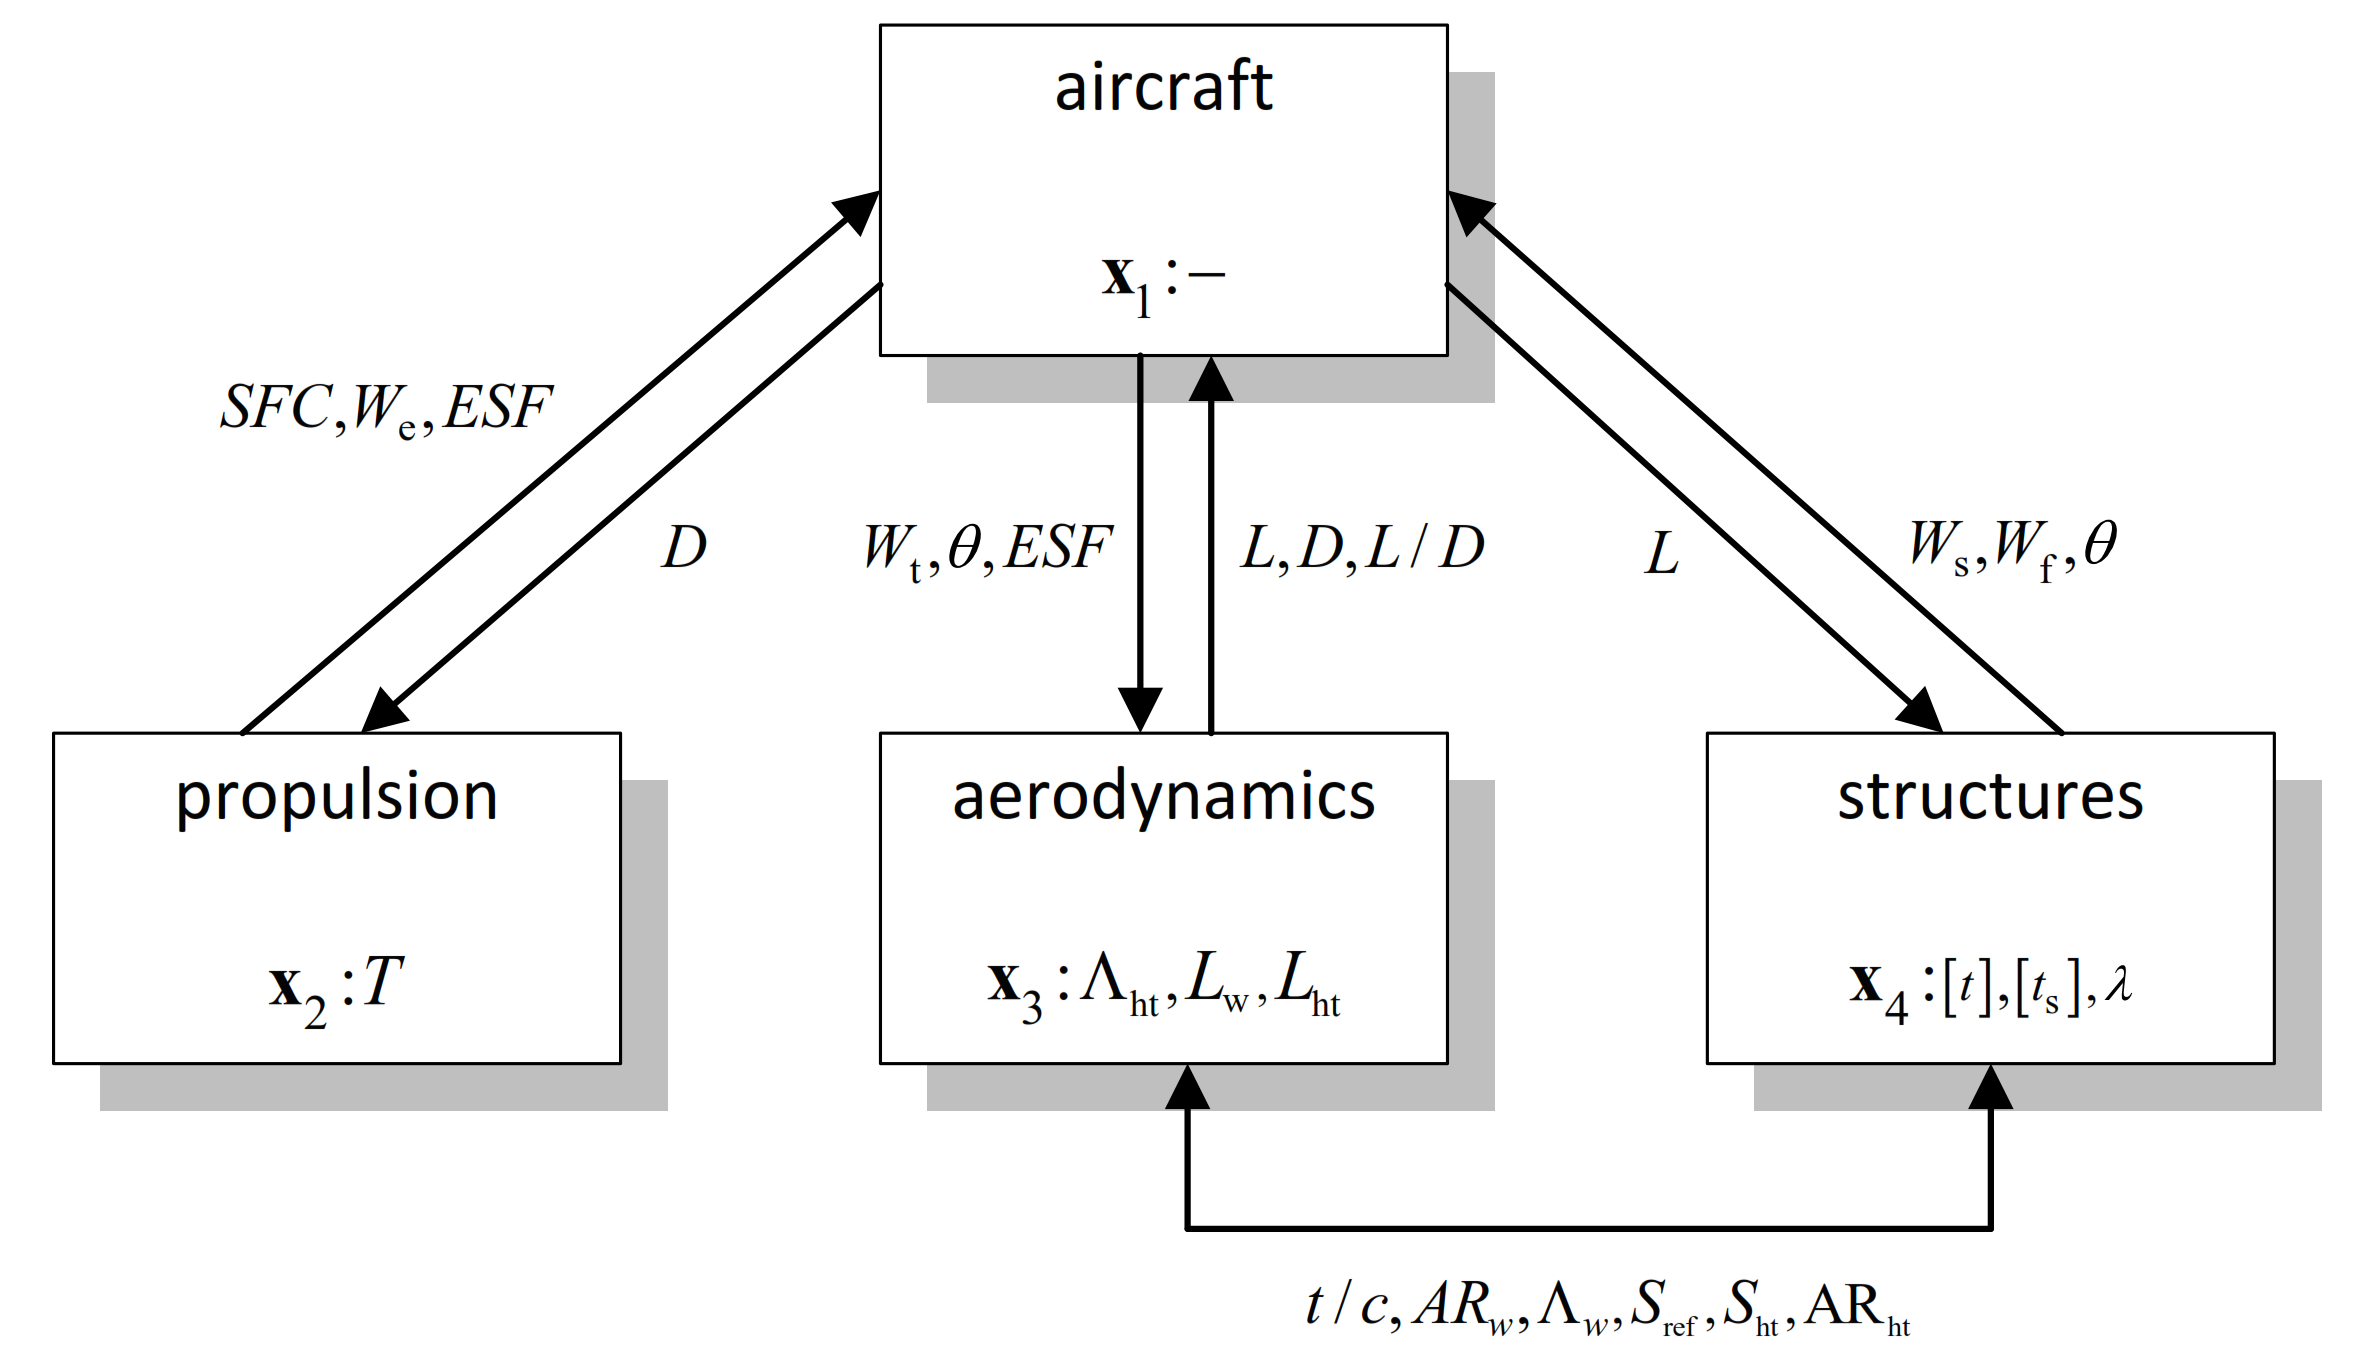
\includegraphics[height=5cm]{images/SBJ_schematics_001.png}
        \end{figure}\strut
    \end{minipage}\tabularnewline
    \begin{minipage}[t]{0.97\columnwidth}\centering
        Fig.1 ATC formulation of SBJ distributed MDO problem\strut
    \end{minipage}\tabularnewline
    \bottomrule
\end{longtable}

All the files defined this formulation are given in the file
\url{SBJ_problem_A.py}. The first subproblem is given below:
\begin{equation*}
    \begin{aligned}
        & \underset{\mathbf{x}}{\text{minimize}}
        & & W_{\mathrm{t}}^{\mathrm{a}}+\phi\left(\mathrm{SFC}^{\mathrm{a}}-\mathrm{SFC}^{\mathrm{p}}\right)+\phi\left(W_{\mathrm{e}}^{\mathrm{a}}-W_{\mathrm{e}}^{\mathrm{p}}\right)+\phi\left(D^{\mathrm{a}}-D^{\mathrm{ae}}\right)+\phi\left(D^{\mathrm{a}}-D^{\mathrm{p}}\right)\\
    & & & +\phi\left(\mathrm{ESF}^{\mathrm{a}}-\mathrm{ESF}^{\mathrm{ae}}\right)+\phi\left(\mathrm{ESF}^{\mathrm{a}}-\mathrm{ESF}^{\mathrm{p}}\right)+\phi\left(W_{\mathrm{t}}^{\mathrm{ae}}-W_{\mathrm{t}}^{\mathrm{a}}\right)+\phi\left(L / D^{\mathrm{a}}-L / D^{\mathrm{ae}}\right) \\
    & & & +\phi\left(t / c^{\mathrm{a}}-t / c^{\mathrm{ae}}\right)+\phi\left(t / c^{\mathrm{a}}-t / c^{\mathrm{s}}\right)+\phi\left(\mathrm{AR}_{\mathrm{w}}^{\mathrm{a}}-\mathrm{AR}_{\mathrm{w}}^{\mathrm{ae}}\right)+\phi\left(\mathrm{AR}_{\mathrm{w}}^{\mathrm{a}}-\mathrm{AR}_{\mathrm{w}}^{\mathrm{s}}\right) \\
    & & & +\phi\left(\Lambda_{\mathrm{w}}^{\mathrm{a}}-\Lambda_{\mathrm{w}}^{\mathrm{ae}}\right)+\phi\left(\Lambda_{\mathrm{w}}^{\mathrm{a}}-\Lambda_{\mathrm{w}}^{\mathrm{s}}\right)+\phi\left(S_{\mathrm{ref}}^{\mathrm{a}}-S_{\mathrm{ref}}^{\mathrm{ae}}\right)+\phi\left(S_{\mathrm{ref}}^{\mathrm{a}}-S_{\mathrm{ref}}^{\mathrm{s}}\right) \\
    & & & +\phi\left(S_{\mathrm{ht}}^{\mathrm{a}}-S_{\mathrm{ht}}^{\mathrm{ae}}\right)+\phi\left(S_{\mathrm{ht}}^{\mathrm{a}}-S_{\mathrm{ht}}^{\mathrm{s}}\right)+\phi\left(\mathrm{AR}_{\mathrm{ht}}^{\mathrm{a}}-\mathrm{AR}_{\mathrm{ht}}^{\mathrm{a}}\right)+\phi\left(\mathrm{AR}_{\mathrm{ht}}^{\mathrm{a}}-\mathrm{AR}_{\mathrm{ht}}^{\mathrm{s}}\right) \\
    & & & +\phi\left(\theta^{\mathrm{a}}-\theta^{\mathrm{ae}}\right)+\phi\left(\theta^{\mathrm{a}}-\theta^{\mathrm{s}}\right)+\phi\left(L^{\mathrm{a}}-L^{\mathrm{ae}}\right)+\phi\left(L^{\mathrm{a}}-L^{\mathrm{s}}\right) \\
    & & & +\phi\left(W_{\mathrm{f}}^{\mathrm{a}}-W_{\mathrm{f}}^{\mathrm{s}}\right)+\phi\left(W_{\mathrm{s}}^{\mathrm{a}}-W_{\mathrm{s}}^{\mathrm{s}}\right) \\
        & \text{subject to}
        & & g_{\mathrm{aircraft}}\left(\mathrm{SFC}^{\mathrm{a}}, W_{\mathrm{e}}^{\mathrm{a}}, L / D^{\mathrm{a}}, W_{\mathrm{f}}^{\mathrm{a}}, W_{\mathrm{s}}^{\mathrm{a}}\right) \leq 0\\
    & \text{while solving}
        & & W_{\mathrm{t}}^{\mathrm{a}}=W_{\mathrm{t}}\left(W_{\mathrm{e}}^{\mathrm{a}}, W_{\mathrm{f}}^{\mathrm{a}}, W_{\mathrm{s}}^{\mathrm{a}}\right)\\
    & \text{where}
        & & \mathbf{x} = \left[\mathrm{SFC}^{\mathrm{a}}, W_{\mathrm{e}}^{\mathrm{a}}, D^{\mathrm{a}}, \mathrm{ESF}^{\mathrm{a}}, L / D^{\mathrm{a}}, t / c^{\mathrm{a}}, \mathrm{AR}_{\mathrm{w}}^{\mathrm{a}}, \Lambda_{\mathrm{w}}^{\mathrm{a}}, S_{\mathrm{ref}}^{\mathrm{a}}, S_{\mathrm{ht}}^{\mathrm{a}}, \mathrm{AR}_{\mathrm{ht}}^{\mathrm{a}}, \theta^{\mathrm{a}}, L^{\mathrm{a}}, W_{\mathrm{f}}^{\mathrm{a}}, W_{\mathrm{s}}^{\mathrm{a}}\right]^\textit{T}
    \end{aligned}
\end{equation*}

The objective/coupling variable \(W_{\mathrm{t}}^{\mathrm{a}}\) is
calculated by \texttt{SBJ\_A1}. The constraint \(g_{\mathrm{aircraft}}\)
and the overall optimization problem are defined in \texttt{SBJ\_opt1}

The second subproblem for the propulsion discipline is given below:

\begin{equation*}
    \begin{aligned}
        & \underset{\mathbf{x}}{\text{minimize}}
        & & \phi\left(\mathrm{SFC}^{\mathrm{a}}-\mathrm{SFC}^{\mathrm{p}}\right)+\phi\left(W_{\mathrm{e}}^{\mathrm{a}}-W_{\mathrm{e}}^{\mathrm{p}}\right)+\phi\left(D^{\mathrm{a}}-D^{\mathrm{p}}\right)+\phi\left(\mathrm{ESF}^{\mathrm{a}}-\mathrm{ESF}^{\mathrm{p}}\right) \\
    & \text{subject to}
        & & \mathrm{g}_{\mathrm{prop}}\left(D^{\mathrm{p}}, T\right) \leq \mathbf{0} \\
    & \text{while solving}
        & & W_{\mathrm{e}}^{\mathrm{p}}=W_{\mathrm{e}}\left(D^{\mathrm{p}}, T\right) \\
    & & & \mathrm{SFC}^{\mathrm{p}}=\operatorname{SFC}\left(D^{\mathrm{p}}, T\right) \\
    & & & \mathrm{ESF}^{\mathrm{p}}=\mathrm{ESF}\left(D^{\mathrm{p}}, T\right) \\
    & \text{where}
        & & \mathbf{x} = \left[D^p,T\right]^\textit{T}
    \end{aligned}
\end{equation*}

The calculation of the coupling variables
\(W_{\mathrm{e}}^{\mathrm{p}}\), \(\mathrm{SFC}^{\mathrm{p}}\), and
\(\mathrm{ESF}^{\mathrm{p}}\), is given by \texttt{SBJ\_A2}. The
calculation of the objective and constraint and definition of the
optimization problem is given by \texttt{SBJ\_opt2}.

The third subproblem for the structural discipline is given below:

\begin{equation*}
    \begin{aligned}
        & \underset{\mathbf{x}}{\text{minimize}}
        & & \phi\left(W_{\mathrm{t}}^{\mathrm{ae}}-W_{\mathrm{t}}^{\mathrm{a}}\right)+\phi\left(t / c^{\mathrm{a}}-t / c^{\mathrm{ae}}\right)+\phi\left(\mathrm{AR}_{\mathrm{w}}^{\mathrm{a}}-\mathrm{AR}_{\mathrm{w}}^{\mathrm{ae}}\right)+\phi\left(\Lambda_{\mathrm{w}}^{\mathrm{a}}-\Lambda_{\mathrm{w}}^{\mathrm{ae}}\right) \\
    & & & +\phi\left(S_{\mathrm{ref}}^{\mathrm{a}}-S_{\mathrm{ref}}^{\mathrm{ae}}\right)+\phi\left(S_{\mathrm{ht}}^{\mathrm{a}}-S_{\mathrm{ht}}^{\mathrm{ae}}\right)+\phi\left(\mathrm{AR}_{\mathrm{ht}}^{\mathrm{a}}-\mathrm{AR}_{\mathrm{ht}}^{\mathrm{ae}}\right)+\phi\left(D^{\mathrm{a}}-D^{\mathrm{ae}}\right) \\
    & & & +\phi\left(\mathrm{ESF}^{\mathrm{a}}-\mathrm{ESF}^{\mathrm{ae}}\right)+\phi\left(L / D^{\mathrm{a}}-L / D^{\mathrm{ae}}\right)+\phi\left(\theta^{\mathrm{a}}-\theta^{\mathrm{ae}}\right)+\phi\left(L^{\mathrm{a}}-L^{\mathrm{ae}}\right)\\
    & \text{subject to}
        & & \mathbf{g}_{\text {aero }}\left(W_{\mathrm{t}}^{\mathrm{ae}}, t / c^{\mathrm{ae}}, \mathrm{AR}_{\mathrm{w}}^{\mathrm{ae}}, \Lambda_{\mathrm{w}}^{\mathrm{ae}}, S_{\mathrm{ref}}^{\mathrm{ae}}, S_{\mathrm{ht}}^{\mathrm{ae}}, \mathrm{AR}_{\mathrm{ht}}^{\mathrm{ae}}, \Lambda_{\mathrm{ht}}, L_{\mathrm{w}}, L_{\mathrm{ht}}, \mathrm{ESF}^{\mathrm{ae}}, \theta^{\mathrm{ae}}\right) \leq \mathbf{0} \\
    & \text{while solving}
        & &   D^{\mathrm{ae}}=D\left(W_{\mathrm{t}}^{\mathrm{ae}}, t / c^{\mathrm{ae}}, \mathrm{AR}_{\mathrm{w}}^{\mathrm{ae}}, \Lambda_{\mathrm{w}}^{\mathrm{ae}}, S_{\mathrm{ref}}^{\mathrm{ae}}, S_{\mathrm{ht}}^{\mathrm{ae}}, \mathrm{AR}_{\mathrm{ht}}^{\mathrm{ae}}, \Lambda_{\mathrm{ht}}, L_{\mathrm{w}}, L_{\mathrm{ht}}, \mathrm{ESF}^{\mathrm{ae}}, \theta^{\mathrm{ae}}\right) \\
    & & & L / D^{\mathrm{ae}}=L / D\left(W_{\mathrm{t}}^{\mathrm{ae}}, t / c^{\mathrm{ae}}, \mathrm{AR}_{\mathrm{w}}^{\mathrm{ae}}, \Lambda_{\mathrm{w}}^{\mathrm{ae}}, S_{\mathrm{ref}}^{\mathrm{ae}}, S_{\mathrm{ht}}^{\mathrm{ae}}, \mathrm{AR}_{\mathrm{ht}}^{\mathrm{ae}}, \Lambda_{\mathrm{ht}}, L_{\mathrm{w}}, L_{\mathrm{ht}}, \mathrm{ESF}^{\mathrm{ae}}, \theta^{\mathrm{ae}}\right) \\
    & & & L^{\mathrm{ae}}=L\left(W_{\mathrm{t}}^{\mathrm{ae}}, t / c^{\mathrm{ae}}, \mathrm{AR}_{\mathrm{w}}^{\mathrm{ae}}, \Lambda_{\mathrm{w}}^{\mathrm{ae}}, S_{\mathrm{ref}}^{\mathrm{ae}}, S_{\mathrm{ht}}^{\mathrm{ae}}, \mathrm{AR}_{\mathrm{ht}}^{\mathrm{ae}}, \Lambda_{\mathrm{ht}}, L_{\mathrm{w}}, L_{\mathrm{ht}}, \mathrm{ESF}^{\mathrm{ae}}, \theta^{\mathrm{ae}}\right)\\
    & \text{where}
        & & \mathbf{x} = \left[W_{\mathrm{t}}^{\mathrm{ae}}, t / c^{\mathrm{ae}}, \mathrm{AR}_{\mathrm{w}}^{\mathrm{ae}}, \Lambda_{\mathrm{w}}^{\mathrm{ae}}, S_{\mathrm{ref}}^{\mathrm{ae}}, S_{\mathrm{ht}}^{\mathrm{ae}}, \mathrm{AR}_{\mathrm{ht}}^{\mathrm{ae}}, \Lambda_{\mathrm{ht}}, L_{\mathrm{w}}, L_{\mathrm{ht}}, \mathrm{ESF}^{\mathrm{ae}}, \theta^{\mathrm{ae}}\right]^\textit{T}
    \end{aligned}
\end{equation*}

There is no local objective. The calculation of the coupling variables
\(D^{\mathrm{ae}}\), \(L / D^{\mathrm{ae}}\), and \(L^{\mathrm{ae}}\),
is given by \texttt{SBJ\_A3}. The calculation of the constraints
\(\mathbf{g}_{\text {prop }}\) and definition of the optimization
problem is given by \texttt{SBJ\_opt3}.

The fourth subproblem for the aerodynamics discipline is given below:

\begin{equation*}
    \begin{aligned}
        & \underset{\mathbf{x}}{\text{minimize}}
        & & \phi\left(t / c^{\mathrm{a}}-t / c^{\mathrm{s}}\right)+\phi\left(\mathrm{AR}_{\mathrm{w}}^{\mathrm{a}}-\mathrm{AR}_{\mathrm{w}}^{\mathrm{s}}\right)+\phi\left(\Lambda_{\mathrm{w}}^{\mathrm{a}}-\Lambda_{\mathrm{w}}^{\mathrm{s}}\right)+\phi\left(S_{\mathrm{ref}}^{\mathrm{a}}-S_{\mathrm{ref}}^{\mathrm{s}}\right) \\
    & & & +\phi\left(S_{\mathrm{ht}}^{\mathrm{a}}-S_{\mathrm{ht}}^{\mathrm{s}}\right)+\phi\left(\mathrm{AR}_{\mathrm{ht}}^{\mathrm{a}}-\mathrm{AR}_{\mathrm{ht}}^{\mathrm{s}}\right)+\phi\left(\theta^{\mathrm{a}}-\theta^{\mathrm{s}}\right)+\phi\left(L^{\mathrm{a}}-L^{\mathrm{s}}\right) \\
    & & & +\phi\left(W_{\mathrm{s}}^{\mathrm{a}}-W_{\mathrm{s}}^{\mathrm{s}}\right)+\phi\left(W_{\mathrm{f}}^{\mathrm{a}}-W_{\mathrm{f}}^{\mathrm{s}}\right) \\
    & \text{subject to}
        & & \mathbf{g}_{\mathrm{struc}}\left(t / c^{\mathrm{s}}, \mathrm{AR}_{\mathrm{w}}^{\mathrm{s}}, \Lambda_{\mathrm{w}}^{\mathrm{s}}, S_{\mathrm{ref}}^{\mathrm{s}}, S_{\mathrm{ht}}^{\mathrm{s}}, \mathrm{AR}_{\mathrm{ht}}^{\mathrm{s}}, L^{\mathrm{s}},[t],\left[t_{\mathrm{s}}\right], \lambda\right) \leq \mathbf{0} \\
    & \text{while solving}
        & &   W_{\mathrm{s}}^{\mathrm{s}}=W_{\mathrm{s}}\left(t / c^{\mathrm{s}}, \mathrm{AR}_{\mathrm{w}}^{\mathrm{s}}, \Lambda_{\mathrm{w}}^{\mathrm{s}}, S_{\mathrm{ref}}^{\mathrm{s}}, S_{\mathrm{ht}}^{\mathrm{s}}, \mathrm{AR}_{\mathrm{ht},}^{\mathrm{s}}, L^{\mathrm{s}},[t],\left[t_{\mathrm{s}}\right], \lambda\right) \\
    & & & W_{\mathrm{f}}^{\mathrm{s}}=W_{\mathrm{f}}\left(t / c^{\mathrm{s}}, \mathrm{AR}_{\mathrm{w}}^{\mathrm{s}}, \Lambda_{\mathrm{w}}^{\mathrm{s}}, S_{\mathrm{ref}}^{\mathrm{s}}, S_{\mathrm{ht}}^{\mathrm{s}}, \mathrm{AR}_{\mathrm{ht}}^{\mathrm{s}}, L^{\mathrm{s}},[t],\left[t_{\mathrm{s}}\right], \lambda\right) \\
    & & & \theta^{\mathrm{s}}=\theta\left(t / c^{\mathrm{s}}, \mathrm{AR}_{\mathrm{w}}^{\mathrm{s}}, \Lambda_{\mathrm{w}}^{\mathrm{s}}, S_{\mathrm{ref}}^{\mathrm{s}}, S_{\mathrm{ht}}^{\mathrm{s}}, \mathrm{AR}_{\mathrm{ht}}^{\mathrm{s}}, L^{\mathrm{s}},[t],\left[t_{\mathrm{s}}\right], \lambda\right)\\
    & \text{where}
        & & \mathbf{x} = \left[t / c^{\mathrm{s}}, \mathrm{AR}_{\mathrm{w}}^{\mathrm{s}}, \Lambda_{\mathrm{w}}^{\mathrm{s}}, S_{\mathrm{ref}}^{\mathrm{s}}, S_{\mathrm{ht}}^{\mathrm{s}}, \mathrm{AR}_{\mathrm{ht}}^{\mathrm{s}}, L^{\mathrm{s}},[t],\left[t_{\mathrm{s}}\right], \lambda\right]^\textit{T}
    \end{aligned}
\end{equation*}

There is no local objective. The calculation of the coupling variables
\(W_{\mathrm{s}}^{\mathrm{s}}\), \(W_{\mathrm{f}}^{\mathrm{s}}\), and
\(\theta^{\mathrm{s}}\), is given by \texttt{SBJ\_A4}. The calculation
of the constraints \(\mathbf{g}_{\mathrm{struc}}\) and definition of the
optimization problem is given by \texttt{SBJ\_opt4}.

The next step is to define all of our optimization variables. To do this
more easily to break up the block diagram to let us easily see how many
variables are associated with each subproblem.

\begin{longtable}[]{@{}c@{}}
    \toprule
    \endhead
    \begin{minipage}[t]{0.97\columnwidth}\centering
        \begin{figure}
            \centering
            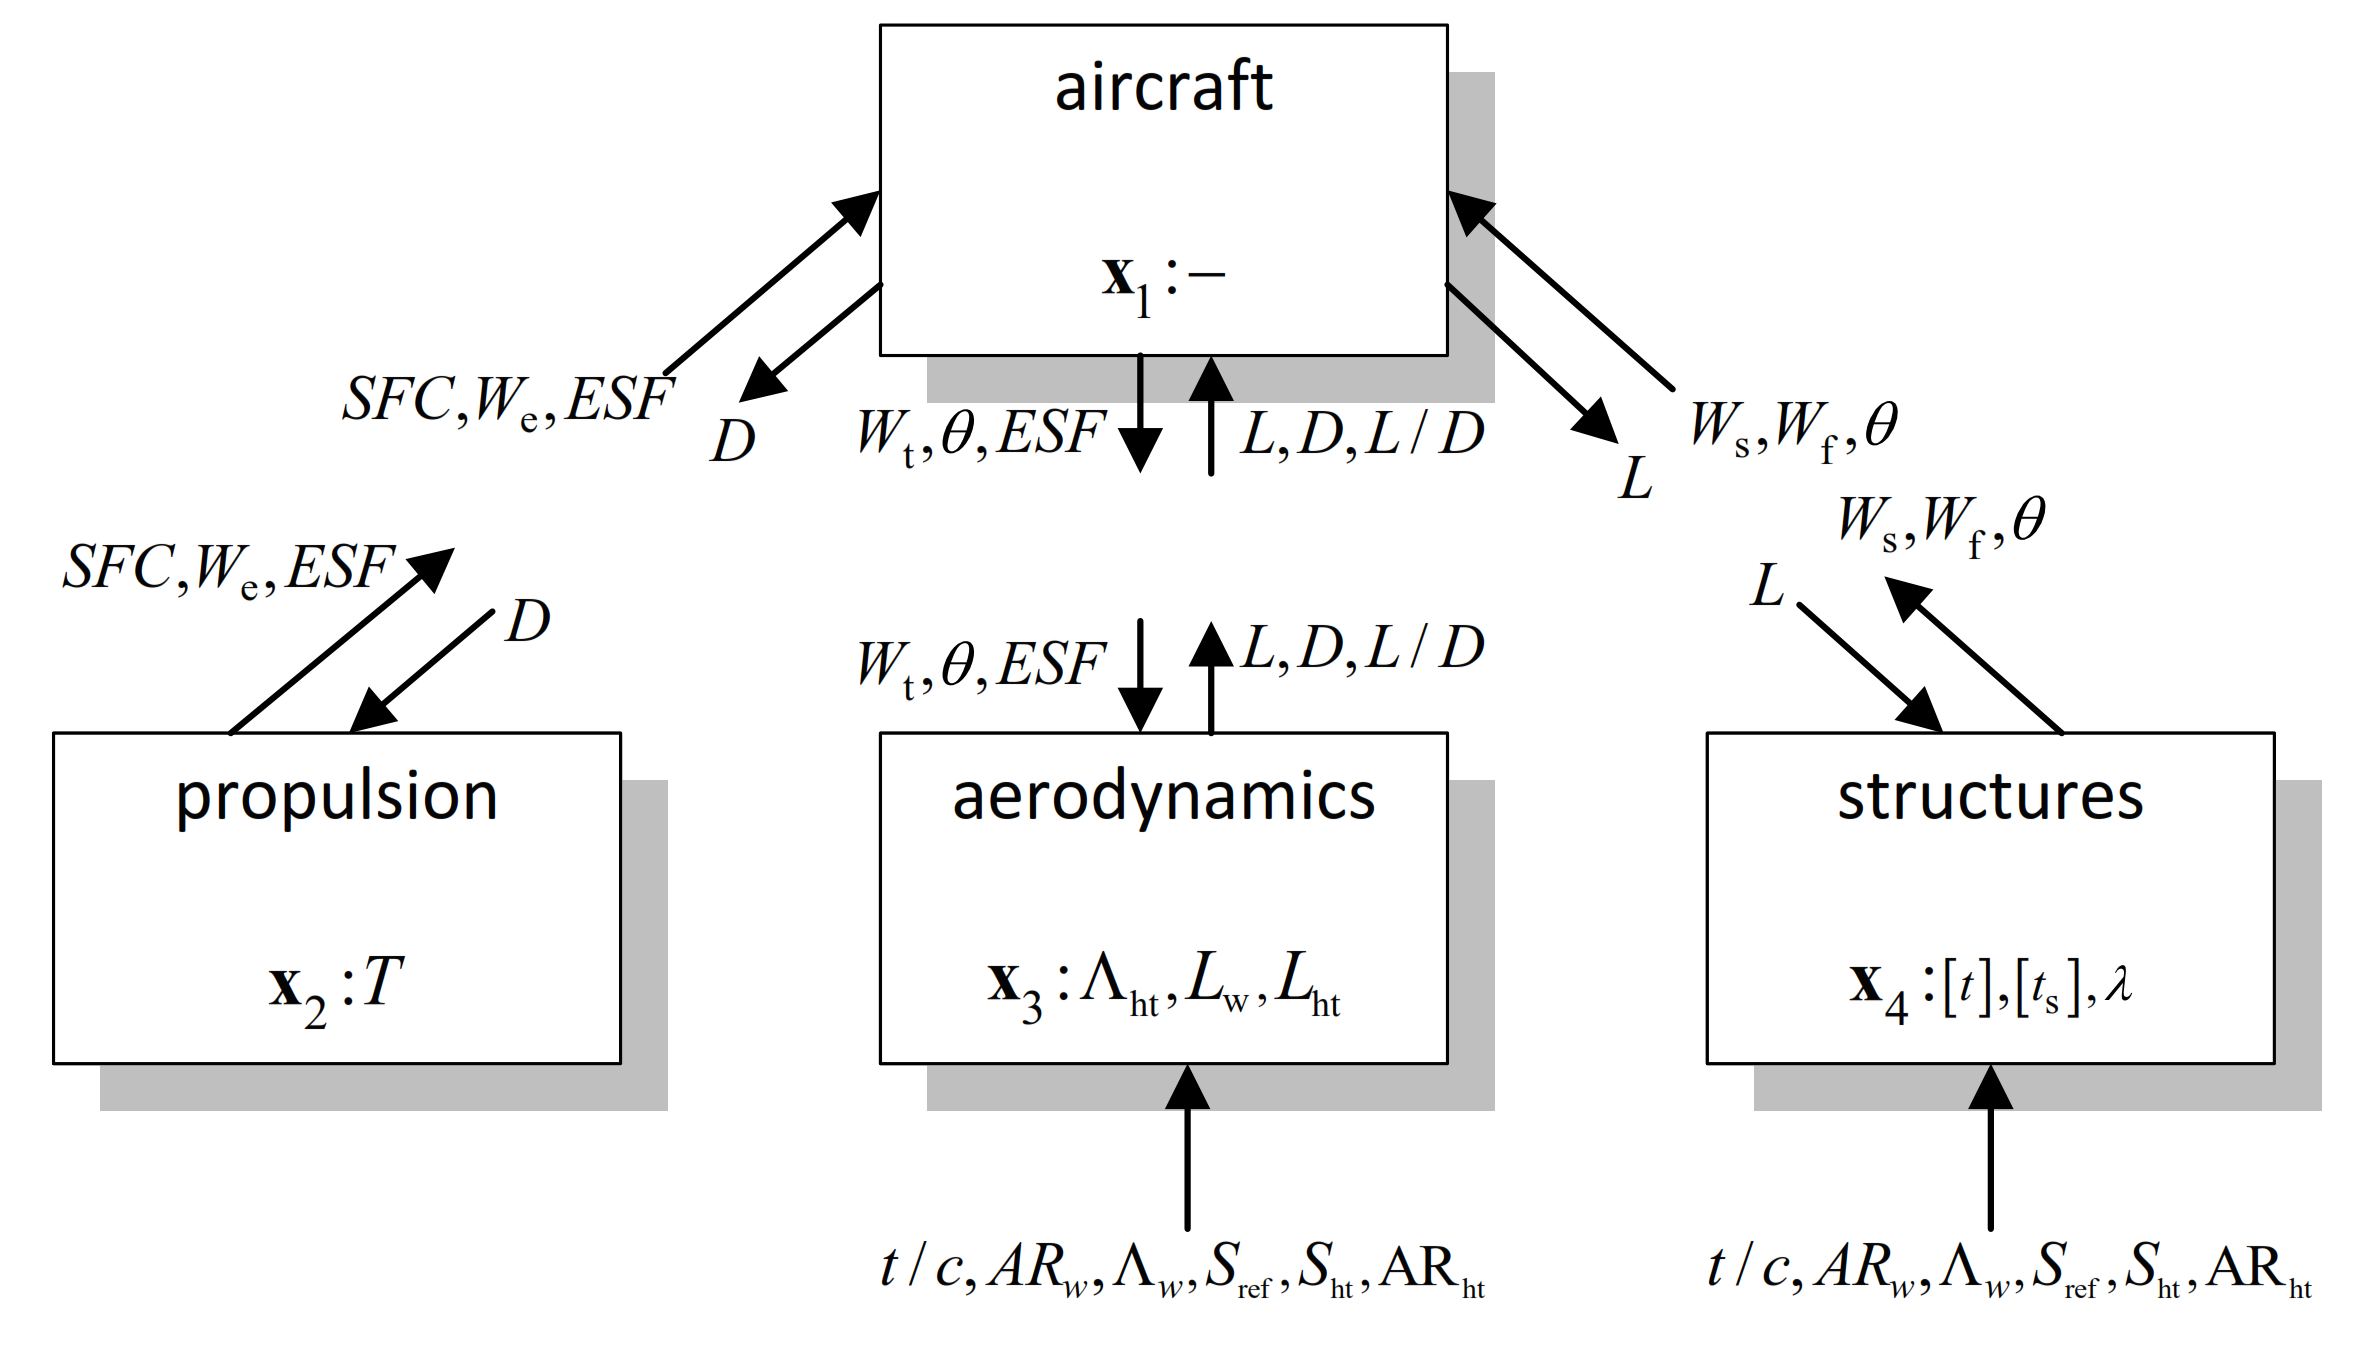
\includegraphics[height=5cm]{images/SBJ_schematics_002.png}
        \end{figure}\strut
    \end{minipage}\tabularnewline
    \begin{minipage}[t]{0.97\columnwidth}\centering
        Fig.2 Breakdown of ATC formulation of SBJ distributed MDO
problem\strut
    \end{minipage}\tabularnewline
    \bottomrule
\end{longtable}

We can now define the properties of each variable in the table below and
code this in \url{SBJ_problem_A.py}. This bookkeeping is the trickiest
part of defining any distributed MDO problem.

\begin{longtable}[]{@{}llllllll@{}}
\toprule
index & subproblem & name & coupling type & link & lower bound & upper
bound & baseline\tabularnewline
\midrule
\endhead
1 & 1 & \texttt{SFC} & feedback & 2 & 1 & 4 & 1.0\tabularnewline
2 & 1 & \texttt{We} & feedback & 2 & 100 & 30000 & 1.0\tabularnewline
3 & 1 & \texttt{ESF} & feedback & 2 & 0.5 & 1.5 & 1.0\tabularnewline
4 & 1 & \texttt{D} & feedforward & 2 & 1000 & 70000 & 1.0\tabularnewline
5 & 1 & \texttt{Wt} & feedforward & 3 & 5000 & 100000 &
1.0\tabularnewline
6 & 1 & \texttt{theta} & feedforward & 3 & 0.2 & 50 & 1.0\tabularnewline
7 & 1 & \texttt{ESF} & feedforward & 3 & 0.5 & 1.5 & 1.0\tabularnewline
8 & 1 & \texttt{L} & feedback & 3 & 5000 & 100000 & 1.0\tabularnewline
9 & 1 & \texttt{D} & feedback & 3 & 1000 & 70000 & 1.0\tabularnewline
10 & 1 & \texttt{LD} & feedback & 3 & 0.1 & 10 & 1.0\tabularnewline
11 & 1 & \texttt{L} & feedforward & 4 & 5000 & 100000 &
1.0\tabularnewline
12 & 1 & \texttt{Ws} & feedback & 4 & 5000 & 100000 & 1.0\tabularnewline
13 & 1 & \texttt{Wf} & feedback & 4 & 5000 & 100000 & 1.0\tabularnewline
14 & 1 & \texttt{theta} & feedback & 4 & 0.2 & 50 & 1.0\tabularnewline
15 & 2 & \texttt{SFC} & feedforward & 1 & 1 & 4 & 1.0\tabularnewline
16 & 2 & \texttt{We} & feedforward & 1 & 100 & 30000 &
1.0\tabularnewline
17 & 2 & \texttt{ESF} & feedforward & 1 & 0.5 & 1.5 & 1.0\tabularnewline
18 & 2 & \texttt{D} & feedback & 1 & 1000 & 70000 & 1.0\tabularnewline
19 & 2 & \texttt{T} & uncoupled & None & 0.1 & 1.0 & 1.0\tabularnewline
20 & 3 & \texttt{Wt} & feedback & 1 & 5000 & 100000 & 1.0\tabularnewline
21 & 3 & \texttt{theta} & feedback & 1 & 0.2 & 50 & 1.0\tabularnewline
22 & 3 & \texttt{ESF} & feedback & 1 & 0.5 & 1.5 & 1.0\tabularnewline
23 & 3 & \texttt{L} & feedforward & 1 & 5000 & 100000 &
1.0\tabularnewline
24 & 3 & \texttt{D} & feedforward & 1 & 1000 & 70000 &
1.0\tabularnewline
25 & 3 & \texttt{LD} & feedforward & 1 & 0.1 & 10 & 1.0\tabularnewline
26 & 3 & \texttt{tc} & shared & 4 & 0.01 & 0.1 & 1.0\tabularnewline
27 & 3 & \texttt{ARw} & shared & 4 & 2.5 & 8.0 & 1.0\tabularnewline
28 & 3 & \texttt{LAMBDAw} & shared & 4 & 40. & 70. & 1.0\tabularnewline
29 & 3 & \texttt{Sref} & shared & 4 & 200. & 800. & 1.0\tabularnewline
30 & 3 & \texttt{Sht} & shared & 4 & 50 & 148.9 & 1.0\tabularnewline
31 & 3 & \texttt{ARht} & shared & 4 & 2.5 & 8.5 & 1.0\tabularnewline
32 & 3 & \texttt{LAMBDAht} & uncoupled & None & 40. & 70. &
1.0\tabularnewline
33 & 3 & \texttt{Lw} & uncoupled & None & 0.01 & 0.2 &
1.0\tabularnewline
34 & 3 & \texttt{Lht} & uncoupled & None & 1 & 3.5 & 1.0\tabularnewline
35 & 4 & \texttt{L} & feedback & 1 & 5000 & 100000 & 1.0\tabularnewline
36 & 4 & \texttt{Ws} & feedforward & 1 & 5000 & 100000 &
1.0\tabularnewline
37 & 4 & \texttt{Wf} & feedforward & 1 & 5000 & 100000 &
1.0\tabularnewline
38 & 4 & \texttt{theta} & feedforward & 1 & 0.2 & 50 &
1.0\tabularnewline
39 & 4 & \texttt{tc} & shared & 3 & 0.01 & 0.1 & 1.0\tabularnewline
40 & 4 & \texttt{ARw} & shared & 3 & 2.5 & 8.0 & 1.0\tabularnewline
41 & 4 & \texttt{LAMBDAw} & shared & 3 & 40. & 70. & 1.0\tabularnewline
42 & 4 & \texttt{Sref} & shared & 3 & 200. & 800. & 1.0\tabularnewline
43 & 4 & \texttt{Sht} & shared & 3 & 50 & 148.9 & 1.0\tabularnewline
44 & 4 & \texttt{ARht} & shared & 3 & 2.5 & 8.5 & 1.0\tabularnewline
45 & 4 & \texttt{lambda} & uncoupled & None & 0.1 & 0.4 &
1.0\tabularnewline
46 & 4 & \texttt{t} & uncoupled & None & 0.1 & 4.0 & 1.0\tabularnewline
47 & 4 & \texttt{t} & uncoupled & None & 0.1 & 4.0 & 1.0\tabularnewline
48 & 4 & \texttt{t} & uncoupled & None & 0.1 & 4.0 & 1.0\tabularnewline
49 & 4 & \texttt{t} & uncoupled & None & 0.1 & 4.0 & 1.0\tabularnewline
50 & 4 & \texttt{t} & uncoupled & None & 0.1 & 4.0 & 1.0\tabularnewline
51 & 4 & \texttt{t} & uncoupled & None & 0.1 & 4.0 & 1.0\tabularnewline
52 & 4 & \texttt{t} & uncoupled & None & 0.1 & 4.0 & 1.0\tabularnewline
53 & 4 & \texttt{t} & uncoupled & None & 0.1 & 4.0 & 1.0\tabularnewline
54 & 4 & \texttt{t} & uncoupled & None & 0.1 & 4.0 & 1.0\tabularnewline
55 & 4 & \texttt{ts} & uncoupled & None & 0.1 & 9.0 & 1.0\tabularnewline
56 & 4 & \texttt{ts} & uncoupled & None & 0.1 & 9.0 & 1.0\tabularnewline
57 & 4 & \texttt{ts} & uncoupled & None & 0.1 & 9.0 & 1.0\tabularnewline
58 & 4 & \texttt{ts} & uncoupled & None & 0.1 & 9.0 & 1.0\tabularnewline
59 & 4 & \texttt{ts} & uncoupled & None & 0.1 & 9.0 & 1.0\tabularnewline
60 & 4 & \texttt{ts} & uncoupled & None & 0.1 & 9.0 & 1.0\tabularnewline
61 & 4 & \texttt{ts} & uncoupled & None & 0.1 & 9.0 & 1.0\tabularnewline
62 & 4 & \texttt{ts} & uncoupled & None & 0.1 & 9.0 & 1.0\tabularnewline
63 & 4 & \texttt{ts} & uncoupled & None & 0.1 & 9.0 & 1.0\tabularnewline
\bottomrule
\end{longtable}

You can follow the remaining steps in the \texttt{SBJ} method of
\url{SBJ_problem_A.py} to fully define all the inputs and outputs needed
by \texttt{DMDO} to solve the problem.

    \begin{tcolorbox}[breakable, size=fbox, boxrule=1pt, pad at break*=1mm,colback=cellbackground, colframe=cellborder]
\prompt{In}{incolor}{1}{\boxspacing}
\begin{Verbatim}[commandchars=\\\{\}]
\PY{k+kn}{from} \PY{n+nn}{SBJ\PYZus{}problem\PYZus{}A} \PY{k+kn}{import} \PY{n}{SBJ}

\PY{n}{MDAO} \PY{o}{=} \PY{n}{SBJ}\PY{p}{(}\PY{p}{)}
\PY{n}{MDAO}\PY{o}{.}\PY{n}{noprogress\PYZus{}stop} \PY{o}{=} \PY{l+m+mi}{5}
\PY{n}{out} \PY{o}{=} \PY{n}{MDAO}\PY{o}{.}\PY{n}{run}\PY{p}{(}\PY{p}{)}
\PY{n+nb}{print}\PY{p}{(}\PY{n}{out}\PY{p}{)}
\end{Verbatim}
\end{tcolorbox}

    \begin{Verbatim}[commandchars=\\\{\}]
c:\textbackslash{}Users\textbackslash{}Khalil\textbackslash{}Desktop\textbackslash{}Documents\textbackslash{}MECH\_559\_material\textbackslash{}MECH559\_notebooks\textbackslash{}.env.win\textbackslash{}l
ib\textbackslash{}site-packages\textbackslash{}OMADS\textbackslash{}POLL.py:103: UserWarning: MS Windows does not support
precision with the \{1e-18\} high resolution of the python numerical library
(numpy) so high precision will be changed to medium precision which supports
\{1e-15\} resolution check: https://numpy.org/doc/stable/user/basics.types.html
  warnings.warn("MS Windows does not support precision with the \{1e-18\} high
resolution of the python numerical library (numpy) so high precision will be
changed to medium precision which supports \{1e-15\} resolution check:
https://numpy.org/doc/stable/user/basics.types.html")
c:\textbackslash{}Users\textbackslash{}Khalil\textbackslash{}Desktop\textbackslash{}Documents\textbackslash{}MECH\_559\_material\textbackslash{}MECH559\_notebooks\textbackslash{}10\_mdo\textbackslash{}SBJ
\_analysis.py:98: RuntimeWarning: invalid value encountered in double\_scalars
  D=np.array([(inputs["Wt"]-CLw1*a-CLht1*b)/1e5, -CLw1*c-CLht1*d])
c:\textbackslash{}Users\textbackslash{}Khalil\textbackslash{}Desktop\textbackslash{}Documents\textbackslash{}MECH\_559\_material\textbackslash{}MECH559\_notebooks\textbackslash{}10\_mdo\textbackslash{}SBJ
\_analysis.py:123: RuntimeWarning: invalid value encountered in double\_scalars
  CL=CLo[0]+CLo[1]
c:\textbackslash{}Users\textbackslash{}Khalil\textbackslash{}Desktop\textbackslash{}Documents\textbackslash{}MECH\_559\_material\textbackslash{}MECH559\_notebooks\textbackslash{}10\_mdo\textbackslash{}SBJ
\_problem\_A.py:82: RuntimeWarning: invalid value encountered in double\_scalars
  g2=(2*(-outputs["CLo2"]))-(outputs["CLo1"])
c:\textbackslash{}Users\textbackslash{}Khalil\textbackslash{}Desktop\textbackslash{}Documents\textbackslash{}MECH\_559\_material\textbackslash{}MECH559\_notebooks\textbackslash{}.env.win\textbackslash{}l
ib\textbackslash{}site-packages\textbackslash{}OMADS\textbackslash{}POLL.py:614: RuntimeWarning: invalid value encountered in
subtract
  return subtract(self.h, other.h, dtype=self.\_dtype.dtype)
c:\textbackslash{}Users\textbackslash{}Khalil\textbackslash{}Desktop\textbackslash{}Documents\textbackslash{}MECH\_559\_material\textbackslash{}MECH559\_notebooks\textbackslash{}10\_mdo\textbackslash{}SBJ
\_problem\_A.py:243: RuntimeWarning: divide by zero encountered in divide
  G1[45:48]=t1/(ts1-.1*t1)-1
c:\textbackslash{}Users\textbackslash{}Khalil\textbackslash{}Desktop\textbackslash{}Documents\textbackslash{}MECH\_559\_material\textbackslash{}MECH559\_notebooks\textbackslash{}10\_mdo\textbackslash{}SBJ
\_problem\_A.py:245: RuntimeWarning: divide by zero encountered in divide
  G1[51:54]=t3/(ts3-.1*t3)-1
c:\textbackslash{}Users\textbackslash{}Khalil\textbackslash{}Desktop\textbackslash{}Documents\textbackslash{}MECH\_559\_material\textbackslash{}MECH559\_notebooks\textbackslash{}10\_mdo\textbackslash{}SBJ
\_problem\_A.py:244: RuntimeWarning: divide by zero encountered in divide
  G1[48:51]=t2/(ts2-.1*t2)-1
    \end{Verbatim}

    \begin{Verbatim}[commandchars=\\\{\}]
0 || qmax: 0.1 || Obj: 10100.0 || dx: 52054.903697188565 || max(w): 1.0
Highest inconsistency : ESF\_2 to ESF\_1
1 || qmax: 0.050176801659138355 || Obj: 10100.0 || dx: 64743.31125307986 ||
max(w): 1.6900000000000002
Highest inconsistency : LD\_3 to LD\_1
2 || qmax: 0.05058899286830934 || Obj: 10100.0 || dx: 73357.89433560152 ||
max(w): 2.8561000000000005
Highest inconsistency : LD\_3 to LD\_1
3 || qmax: 0.051001184077480326 || Obj: 10100.0 || dx: 77123.36702025778 ||
max(w): 4.826809000000002
Highest inconsistency : LAMBDAw\_4 to LAMBDAw\_3
4 || qmax: 0.051413375286651325 || Obj: 10100.0 || dx: 79782.63046025684 ||
max(w): 8.157307210000004
Highest inconsistency : ARw\_4 to ARw\_3
5 || qmax: 0.051825566495822296 || Obj: 10100.0 || dx: 79819.40609956994 ||
max(w): 13.785849184900009
Highest inconsistency : ARw\_4 to ARw\_3
6 || qmax: 0.052237757704993296 || Obj: 10100.0 || dx: 79255.85121053552 ||
max(w): 23.298085122481016
Highest inconsistency : ESF\_3 to ESF\_1
7 || qmax: 0.05264994891416427 || Obj: 10100.0 || dx: 78396.26575620582 ||
max(w): 39.37376385699292
Highest inconsistency : ESF\_3 to ESF\_1
8 || qmax: 0.05264994891416427 || Obj: 10100.0 || dx: 77490.4688953086 ||
max(w): 66.54166091831804
Highest inconsistency : ESF\_3 to ESF\_1
Stop: no progress after 5 iterations.
[-0.00282766 -0.01607554 -0.00783028 -0.0027087  -0.01816632  0.
  0.05       -0.00144316 -0.00135339  0.01103711 -0.00527895 -0.01526209
 -0.05264995  0.00040161  0.          0.01818182  0.01333333 -0.01416667
  0.          0.        ]
    \end{Verbatim}

    \begin{Verbatim}[commandchars=\\\{\}]
c:\textbackslash{}Users\textbackslash{}Khalil\textbackslash{}Desktop\textbackslash{}Documents\textbackslash{}MECH\_559\_material\textbackslash{}MECH559\_notebooks\textbackslash{}.env.win\textbackslash{}l
ib\textbackslash{}site-packages\textbackslash{}DMDO\textbackslash{}DMDO.py:842: RuntimeWarning: divide by zero encountered in
log
  if iter > i + 2 and np.log(np.min(self.Coordinator.w) > 6.) and
np.less\_equal(self.tab\_inc[iter-i], np.min(self.tab\_inc[iter-i+1:iter])):
    \end{Verbatim}

    Let us print all the optimization variables

    \begin{tcolorbox}[breakable, size=fbox, boxrule=1pt, pad at break*=1mm,colback=cellbackground, colframe=cellborder]
\prompt{In}{incolor}{2}{\boxspacing}
\begin{Verbatim}[commandchars=\\\{\}]
\PY{k+kn}{import} \PY{n+nn}{numpy} \PY{k}{as} \PY{n+nn}{np}
\PY{n+nb}{print}\PY{p}{(}\PY{l+s+sa}{f}\PY{l+s+s1}{\PYZsq{}}\PY{l+s+s1}{\PYZhy{}\PYZhy{}\PYZhy{}\PYZhy{}\PYZhy{}\PYZhy{}Run\PYZus{}Summary\PYZhy{}\PYZhy{}\PYZhy{}\PYZhy{}\PYZhy{}\PYZhy{}}\PY{l+s+s1}{\PYZsq{}}\PY{p}{)}
\PY{n+nb}{print}\PY{p}{(}\PY{n}{MDAO}\PY{o}{.}\PY{n}{stop}\PY{p}{)}
\PY{n+nb}{print}\PY{p}{(}\PY{l+s+sa}{f}\PY{l+s+s1}{\PYZsq{}}\PY{l+s+s1}{q = }\PY{l+s+si}{\PYZob{}}\PY{n}{MDAO}\PY{o}{.}\PY{n}{Coordinator}\PY{o}{.}\PY{n}{q}\PY{l+s+si}{\PYZcb{}}\PY{l+s+s1}{\PYZsq{}}\PY{p}{)}
\PY{n}{index} \PY{o}{=} \PY{n}{np}\PY{o}{.}\PY{n}{argmax}\PY{p}{(}\PY{n}{MDAO}\PY{o}{.}\PY{n}{Coordinator}\PY{o}{.}\PY{n}{q}\PY{p}{)}
\PY{k}{for} \PY{n}{i} \PY{o+ow}{in} \PY{n}{MDAO}\PY{o}{.}\PY{n}{Coordinator}\PY{o}{.}\PY{n}{master\PYZus{}vars}\PY{p}{:}
    \PY{n+nb}{print}\PY{p}{(}\PY{l+s+sa}{f}\PY{l+s+s1}{\PYZsq{}}\PY{l+s+si}{\PYZob{}}\PY{n}{i}\PY{o}{.}\PY{n}{name}\PY{l+s+si}{\PYZcb{}}\PY{l+s+s1}{\PYZus{}}\PY{l+s+si}{\PYZob{}}\PY{n}{i}\PY{o}{.}\PY{n}{sp\PYZus{}index}\PY{l+s+si}{\PYZcb{}}\PY{l+s+s1}{ = }\PY{l+s+si}{\PYZob{}}\PY{n}{i}\PY{o}{.}\PY{n}{value}\PY{l+s+si}{\PYZcb{}}\PY{l+s+s1}{\PYZsq{}}\PY{p}{)}
\end{Verbatim}
\end{tcolorbox}

    \begin{Verbatim}[commandchars=\\\{\}]
------Run\_Summary------
No progress after several iterations
q = [-0.00282766 -0.01607554 -0.00783028 -0.0027087  -0.01816632  0.
  0.05       -0.00144316 -0.00135339  0.01103711 -0.00527895 -0.01526209
 -0.05264995  0.00040161  0.          0.01818182  0.01333333 -0.01416667
  0.          0.        ]
SFC\_1 = 1.0
We\_1 = 100.0
ESF\_1 = 0.5
D\_1 = 1.0
Wt\_1 = 10100.0
theta\_1 = 1.0
ESF\_1 = 1.0
L\_1 = 25987.0
D\_1 = 9672.0
LD\_1 = 3.6484375
L\_1 = 1.0
Ws\_1 = 5000.0
Wf\_1 = 5000.0
theta\_1 = 0.2
SFC\_2 = 1.0848297375304163
We\_2 = 4906.587643706783
ESF\_2 = 0.5783028203859475
D\_2 = 1870.0
T\_2 = 0.1
Wt\_3 = 27358.0
theta\_3 = 1.0
ESF\_3 = 0.5
L\_3 = 27358.0
D\_3 = 10605.842079414004
LD\_3 = 2.5557638109850185
tc\_3 = 0.1
ARw\_3 = 3.5
LAMBDAw\_3 = 44.0
Sref\_3 = 627.0
Sht\_3 = 148.9
ARht\_3 = 2.5
LAMBDAht\_3 = 70.0
Lw\_3 = 0.01
Lht\_3 = 3.5
L\_4 = 5016.0
Ws\_4 = 19498.988148878656
Wf\_4 = 55017.45146845605
theta\_4 = 0.0
tc\_4 = 0.1
ARw\_4 = 2.5
LAMBDAw\_4 = 40.0
Sref\_4 = 712.0
Sht\_4 = 148.9
ARht\_4 = 2.5
lambda\_4 = 0.1
t\_4 = 4.0
t\_4 = 1.0
t\_4 = 0.1
t\_4 = 0.1
t\_4 = 4.0
t\_4 = 4.0
t\_4 = 4.0
t\_4 = 0.1
t\_4 = 0.1
ts\_4 = 0.1
ts\_4 = 2.0
ts\_4 = 1.0
ts\_4 = 1.0
ts\_4 = 9.0
ts\_4 = 9.0
ts\_4 = 0.1
ts\_4 = 9.0
ts\_4 = 9.0
range\_1 = 2000.4357977414625
Temp\_E\_2 = 1.1019125000000003
Throttle\_uA\_2 = 3176.2401155565603
Pg\_3 = 0.95
CLo1\_3 = 0.1674121413072983
CLo2\_3 = -0.0020141497188846985
    \end{Verbatim}

    and print the objective \texttt{fmin} and constraint violation
\texttt{hmin}

    \begin{tcolorbox}[breakable, size=fbox, boxrule=1pt, pad at break*=1mm,colback=cellbackground, colframe=cellborder]
\prompt{In}{incolor}{3}{\boxspacing}
\begin{Verbatim}[commandchars=\\\{\}]
\PY{n}{fmin} \PY{o}{=} \PY{l+m+mi}{0}
\PY{n}{hmax} \PY{o}{=} \PY{o}{\PYZhy{}}\PY{n}{np}\PY{o}{.}\PY{n}{inf}
\PY{k}{for} \PY{n}{j} \PY{o+ow}{in} \PY{n+nb}{range}\PY{p}{(}\PY{n+nb}{len}\PY{p}{(}\PY{n}{MDAO}\PY{o}{.}\PY{n}{subProblems}\PY{p}{)}\PY{p}{)}\PY{p}{:}

    \PY{n}{fmin} \PY{o}{=} \PY{n}{MDAO}\PY{o}{.}\PY{n}{subProblems}\PY{p}{[}\PY{n}{j}\PY{p}{]}\PY{o}{.}\PY{n}{MDA\PYZus{}process}\PY{o}{.}\PY{n}{getOutputs}\PY{p}{(}\PY{p}{)}
    \PY{n}{hmin} \PY{o}{=} \PY{n}{MDAO}\PY{o}{.}\PY{n}{subProblems}\PY{p}{[}\PY{n}{j}\PY{p}{]}\PY{o}{.}\PY{n}{opt}\PY{p}{(}\PY{p}{[}\PY{n}{s}\PY{o}{.}\PY{n}{value} \PY{k}{for} \PY{n}{s} \PY{o+ow}{in} \PY{n}{MDAO}\PY{o}{.}\PY{n}{subProblems}\PY{p}{[}\PY{n}{j}\PY{p}{]}\PY{o}{.}\PY{n}{get\PYZus{}design\PYZus{}vars}\PY{p}{(}\PY{p}{)}\PY{p}{]} \PY{p}{,} \PY{n}{MDAO}\PY{o}{.}\PY{n}{subProblems}\PY{p}{[}\PY{n}{j}\PY{p}{]}\PY{o}{.}\PY{n}{MDA\PYZus{}process}\PY{o}{.}\PY{n}{getOutputs}\PY{p}{(}\PY{p}{)}\PY{p}{)}\PY{p}{[}\PY{l+m+mi}{1}\PY{p}{]}

    \PY{n+nb}{print}\PY{p}{(}\PY{l+s+sa}{f}\PY{l+s+s1}{\PYZsq{}}\PY{l+s+s1}{SP\PYZus{}}\PY{l+s+si}{\PYZob{}}\PY{n}{MDAO}\PY{o}{.}\PY{n}{subProblems}\PY{p}{[}\PY{n}{j}\PY{p}{]}\PY{o}{.}\PY{n}{index}\PY{l+s+si}{\PYZcb{}}\PY{l+s+s1}{: fmin= }\PY{l+s+si}{\PYZob{}}\PY{n}{fmin}\PY{l+s+si}{\PYZcb{}}\PY{l+s+s1}{), hmin= }\PY{l+s+si}{\PYZob{}}\PY{n}{hmin}\PY{l+s+si}{\PYZcb{}}\PY{l+s+s1}{\PYZsq{}}\PY{p}{)}
    \PY{k}{if} \PY{n}{MDAO}\PY{o}{.}\PY{n}{subProblems}\PY{p}{[}\PY{n}{j}\PY{p}{]}\PY{o}{.}\PY{n}{is\PYZus{}main}\PY{p}{:}
        \PY{n}{fmin} \PY{o}{=} \PY{n}{MDAO}\PY{o}{.}\PY{n}{subProblems}\PY{p}{[}\PY{n}{j}\PY{p}{]}\PY{o}{.}\PY{n}{MDA\PYZus{}process}\PY{o}{.}\PY{n}{getOutputs}\PY{p}{(}\PY{p}{)}
        \PY{n}{hmin} \PY{o}{=} \PY{n}{MDAO}\PY{o}{.}\PY{n}{subProblems}\PY{p}{[}\PY{n}{j}\PY{p}{]}\PY{o}{.}\PY{n}{opt}\PY{p}{(}\PY{p}{[}\PY{n}{s}\PY{o}{.}\PY{n}{value} \PY{k}{for} \PY{n}{s} \PY{o+ow}{in} \PY{n}{MDAO}\PY{o}{.}\PY{n}{subProblems}\PY{p}{[}\PY{n}{j}\PY{p}{]}\PY{o}{.}\PY{n}{get\PYZus{}design\PYZus{}vars}\PY{p}{(}\PY{p}{)}\PY{p}{]} \PY{p}{,} \PY{n}{MDAO}\PY{o}{.}\PY{n}{subProblems}\PY{p}{[}\PY{n}{j}\PY{p}{]}\PY{o}{.}\PY{n}{MDA\PYZus{}process}\PY{o}{.}\PY{n}{getOutputs}\PY{p}{(}\PY{p}{)}\PY{p}{)}\PY{p}{[}\PY{l+m+mi}{1}\PY{p}{]}
        \PY{k}{if} \PY{n+nb}{max}\PY{p}{(}\PY{n}{hmin}\PY{p}{)} \PY{o}{\PYZgt{}} \PY{n}{hmax}\PY{p}{:}
            \PY{n}{hmax} \PY{o}{=} \PY{n+nb}{max}\PY{p}{(}\PY{n}{hmin}\PY{p}{)}
\PY{n+nb}{print}\PY{p}{(}\PY{l+s+sa}{f}\PY{l+s+s1}{\PYZsq{}}\PY{l+s+s1}{P\PYZus{}main: fmin= }\PY{l+s+si}{\PYZob{}}\PY{n}{fmin}\PY{l+s+si}{\PYZcb{}}\PY{l+s+s1}{, hmax= }\PY{l+s+si}{\PYZob{}}\PY{n}{hmax}\PY{l+s+si}{\PYZcb{}}\PY{l+s+s1}{\PYZsq{}}\PY{p}{)}
\PY{n+nb}{print}\PY{p}{(}\PY{l+s+sa}{f}\PY{l+s+s1}{\PYZsq{}}\PY{l+s+s1}{Final obj value of the main problem: }\PY{l+s+se}{\PYZbs{}n}\PY{l+s+s1}{ }\PY{l+s+si}{\PYZob{}}\PY{n}{fmin}\PY{l+s+si}{\PYZcb{}}\PY{l+s+s1}{\PYZsq{}}\PY{p}{)}
\end{Verbatim}
\end{tcolorbox}

    \begin{Verbatim}[commandchars=\\\{\}]
SP\_1: fmin= [10100.0, 2000.4357977414625]), hmin= [-0.00021789887073131453]
SP\_2: fmin= [1.0848297375304163, 4906.587643706783, 0.5783028203859475,
1.1019125000000003, 3176.2401155565603]), hmin= [0.08030637254901984,
-0.49097047415236283]
SP\_3: fmin= [27358.0, 10605.842079414004, 2.5557638109850185, 0.95,
0.1674121413072983, -0.0020141497188846985]), hmin= [-0.13636363636363646,
-0.1714404407450677, -0.16338384186952892]
SP\_4: fmin= [19498.988148878656, 55017.45146845605, 0.0]), hmin=
[-0.8764347595275616, -0.9972624621169462, -0.9965194094409014,
-0.9903861821266253, -0.9999919171581595, -0.9999952394444181,
-0.9955484948477437, -1.0000080828260998, -1.000004760555399, -0.99868047482447,
-0.9960448984190235, -0.9821775696762981, -0.9899819862571839,
-0.9486807224293599, -0.6490478267537039, -1.010004268530427,
-1.0507415635742832, -1.2355141818066935, -0.8770312053232145,
-0.9972731124175309, -0.9965214620263639, -0.9904539130266758,
-0.9999919171582353, -0.999995239444419, -0.9956162257477942,
-1.0000080828261755, -1.0000047605553999, -0.7879097506678737,
-0.9896131830949869, -0.9961268892609935, -0.99868047482447,
-0.9633613759467613, -0.9821775696762981, -1.010004268530427,
-1.1201400189610216, -1.014600165459527, -0.9899819862571839,
-0.8687046836794554, -0.9851079045644761, -0.9655525478234457,
-0.9904841007663332, -0.996721802582451, -0.9969732157051322,
-0.6892103057634813, -0.3943318251002417, -14.333333333333332,
-0.4736842105263158, -0.898989898989899, -0.898989898989899,
-0.5348837209302326, -0.5348837209302326, -14.333333333333332,
-0.9888765294771968, -0.9888765294771968, -1.1235652404724383,
-1.0027375378830536, -1.0034805905590984, -1.00131952517553,
-1.0039551015809765, -1.0178224303237018, -1.1229687946767855,
-1.002726887582469, -1.0034785379736362, -1.2120902493321264,
-1.010386816905013, -1.0038731107390064, -1.00131952517553, -1.0366386240532388,
-1.0178224303237018, -1.0344474521765543, -1.0095158992336668,
-1.0032781974175489]
P\_main: fmin= [19498.988148878656, 55017.45146845605, 0.0], hmax=
-0.00021789887073131453
Final obj value of the main problem:
 [19498.988148878656, 55017.45146845605, 0.0]
    \end{Verbatim}

    \hypertarget{formulation-b-nhatc}{%
\subsection{Formulation (B): NHATC}\label{formulation-b-nhatc}}

Formulation B is a non-hierarchal one shown below. The overall objective
and constraints are the same as Formulation A and are also given by
discipline 1, \emph{aircraft}.

\begin{longtable}[]{@{}c@{}}
    \toprule
    \endhead
    \begin{minipage}[t]{0.97\columnwidth}\centering
        \begin{figure}
            \centering
            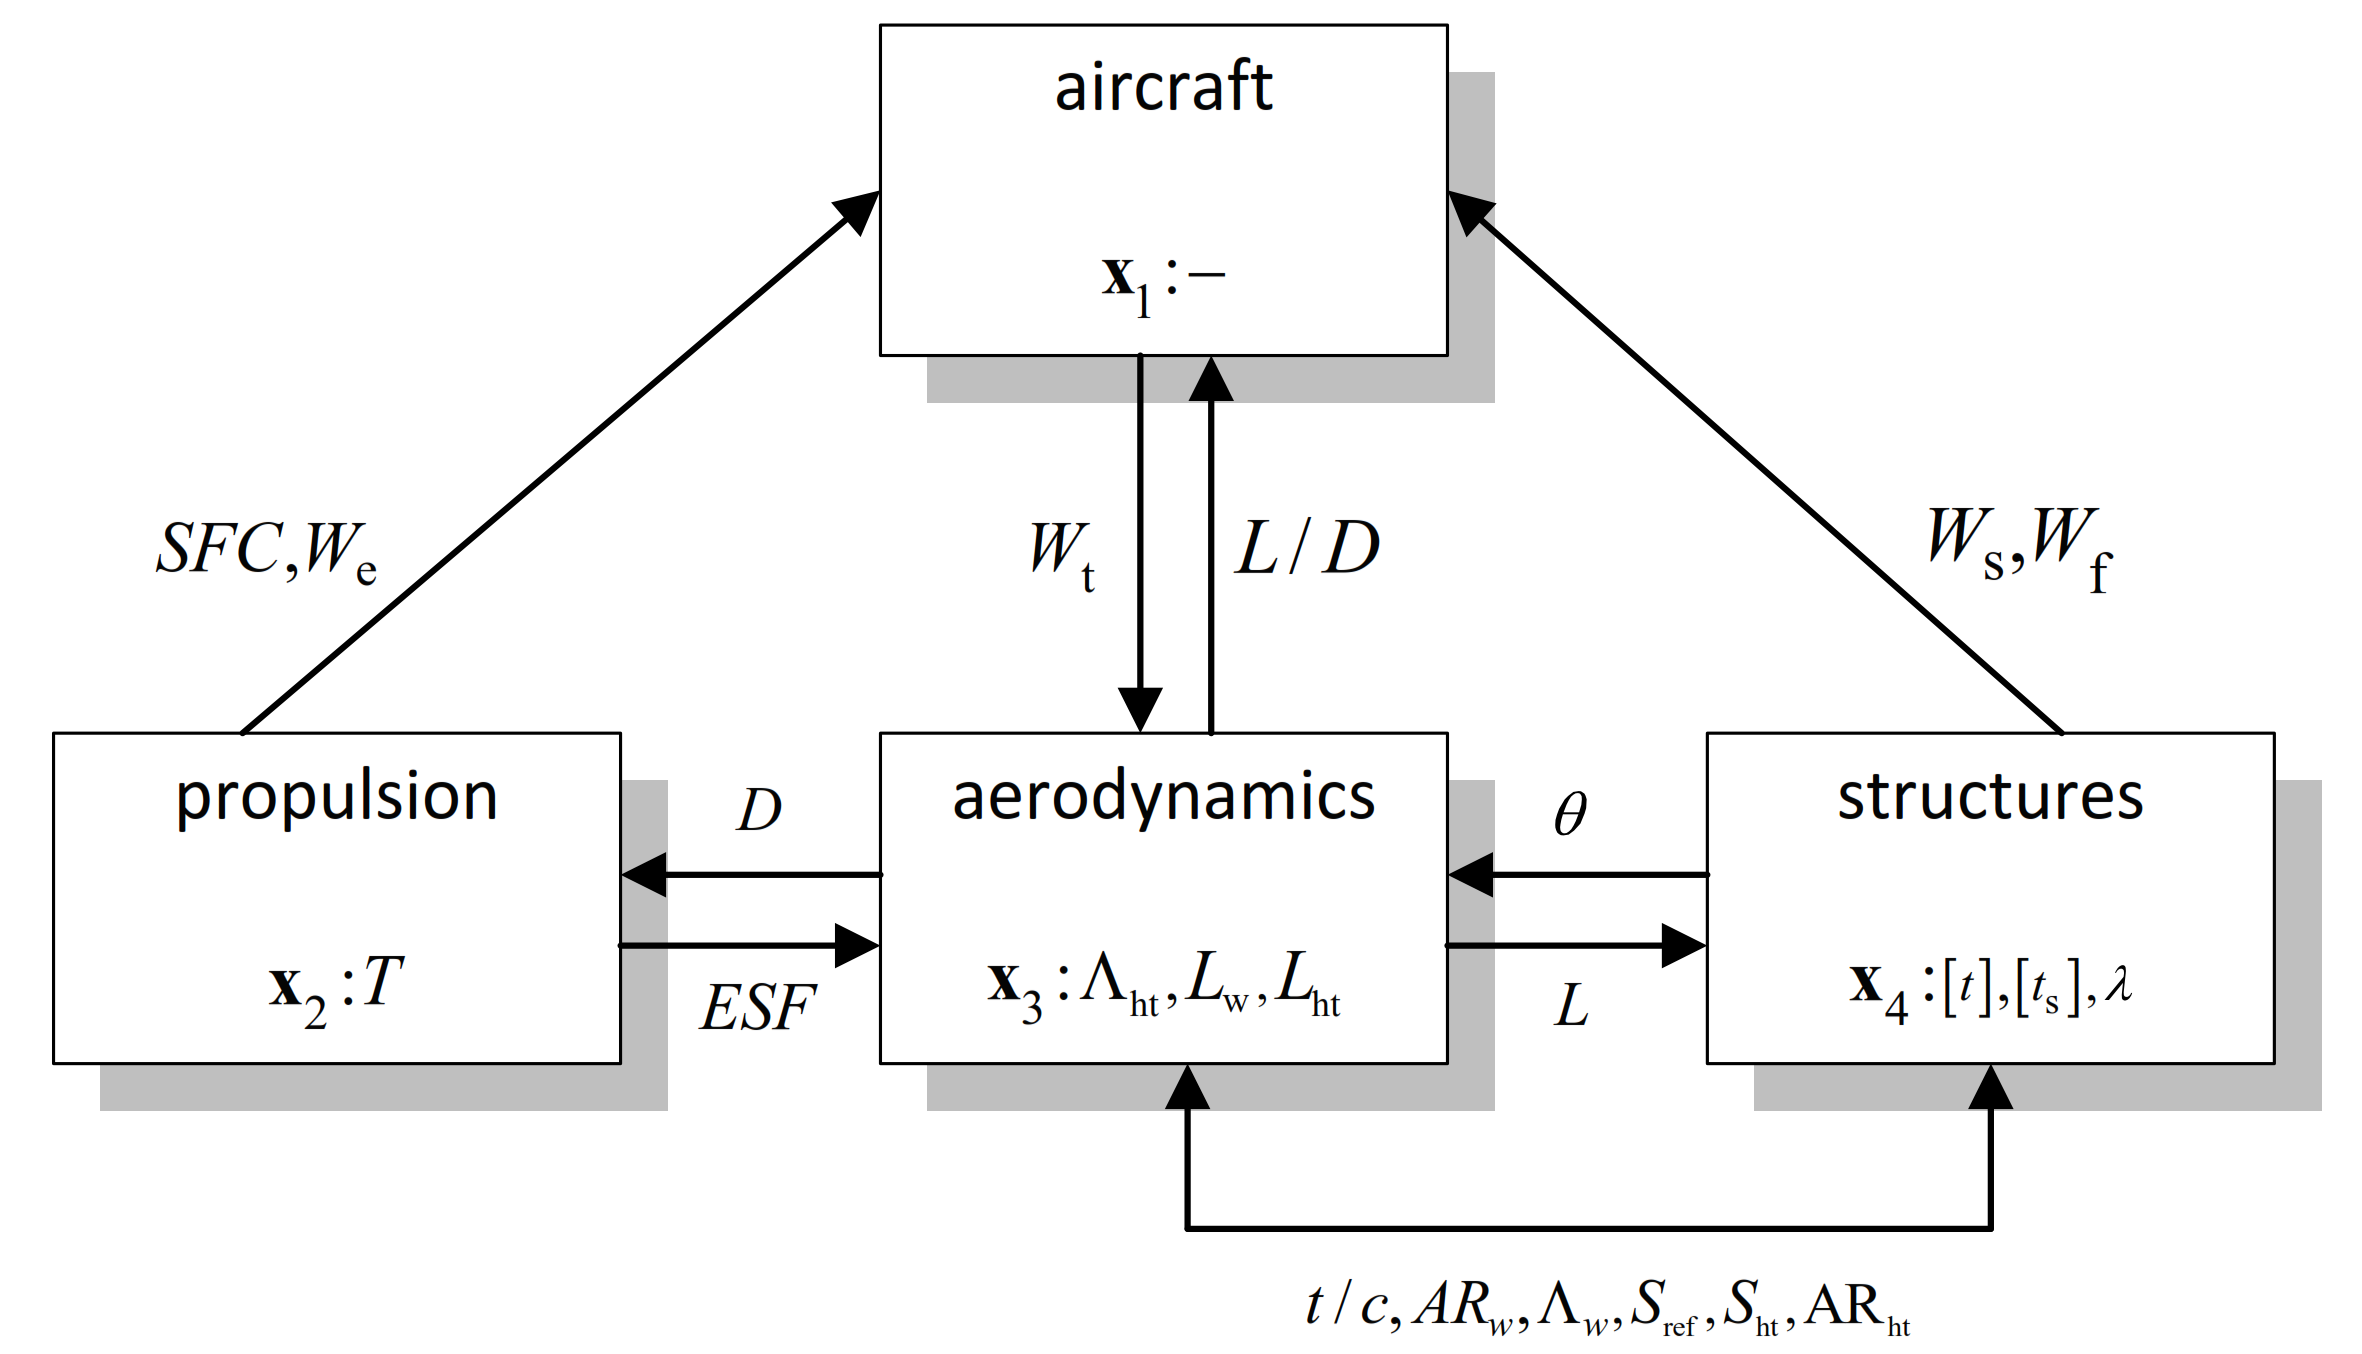
\includegraphics[height=5cm]{images/SBJ_schematics_003.png}
        \end{figure}\strut
    \end{minipage}\tabularnewline
    \begin{minipage}[t]{0.97\columnwidth}\centering
        Fig.3 NHATC formulation of SBJ distributed MDO problem
problem\strut
    \end{minipage}\tabularnewline
    \bottomrule
\end{longtable}

All the files defined this formulation are given in the file
\url{SBJ_problem_B.py}. The first subproblem is given below:
\begin{equation*}
    \begin{aligned}
        & \underset{\mathbf{x}}{\text{minimize}}
        & & W_{\mathrm{t}}^{\mathrm{a}}+\phi\left(\mathrm{SFC}^{\mathrm{a}}-\mathrm{SFC}^{\mathrm{p}}\right)+\phi\left(W_{\mathrm{e}}^{\mathrm{a}}-W_{\mathrm{e}}^{\mathrm{p}}\right)\\
    & & & +\phi\left(L / D^{\mathrm{a}}-L / D^{\mathrm{ae}}\right)+\phi\left(W_{\mathrm{t}}^{\mathrm{ae}}-W_{\mathrm{t}}^{\mathrm{a}}\right)+\phi\left(W_{\mathrm{s}}^{\mathrm{a}}-W_{\mathrm{s}}^{\mathrm{s}}\right)+\phi\left(W_{\mathrm{f}}^{\mathrm{a}}-W_{\mathrm{f}}^{\mathrm{s}}\right) \\
        & \text{subject to}
        & & g_{\text {aircraft }}\left(\mathrm{SFC}^{\mathrm{a}}, W_{\mathrm{e}}^{\mathrm{a}}, L / D^{\mathrm{a}}, W_{\mathrm{f}}^{\mathrm{a}}, W_{\mathrm{s}}^{\mathrm{a}}\right) \leq \mathbf{0} \\
    & \text{while solving}
        & & W_{\mathrm{t}}^{\mathrm{a}}=W_{\mathrm{t}}\left(W_{\mathrm{e}}^{\mathrm{a}}, W_{\mathrm{f}}^{\mathrm{a}}, W_{\mathrm{s}}^{\mathrm{a}}\right)\\
    & \text{where}
        & & \mathbf{x} = \left[\mathrm{SFC}^{\mathrm{a}}, W_{\mathrm{e}}^{\mathrm{a}}, L / D^{\mathrm{a}}, W_{\mathrm{s}}^{\mathrm{a}}, W_{\mathrm{f}}^{\mathrm{a}}\right]^\textit{T}
    \end{aligned}
\end{equation*}

The objective/coupling variable \(W_{\mathrm{t}}^{\mathrm{a}}\) is
calculated by \texttt{SBJ\_A1}. The constraint \(g_{\mathrm{aircraft}}\)
and the overall optimization problem are defined in \texttt{SBJ\_opt1}

The second subproblem for the propulsion discipline is given below:

\begin{equation*}
    \begin{aligned}
        & \underset{\mathbf{x}}{\text{minimize}}
        & & \phi\left(\mathrm{SFC}^{\mathrm{a}}-\mathrm{SFC}^{\mathrm{p}}\right)+\phi\left(W_{\mathrm{e}}^{\mathrm{a}}-W_{\mathrm{e}}^{\mathrm{p}}\right)+\phi\left(D^{\mathrm{p}}-D^{\mathrm{ae}}\right)+\phi\left(\mathrm{ESF}^{\mathrm{ae}}-\mathrm{ESF}^{\mathrm{p}}\right) \\
    & \text{subject to}
        & & \mathbf{g}_{\text {prop }}\left(D^{\mathrm{p}}, T\right) \leq \mathbf{0} \\
    & \text{while solving}
        & & W_{\mathrm{e}}^{\mathrm{p}}=W_{\mathrm{e}}\left(D^{\mathrm{p}}, T\right) \\
    & & & \mathrm{SFC}^{\mathrm{p}}=\operatorname{SFC}\left(D^{\mathrm{p}}, T\right) \\
    & & & \mathrm{ESF}^{\mathrm{p}}=\operatorname{ESF}\left(D^{\mathrm{p}}, T\right) \\
    & \text{where}
        & & \mathbf{x} = \left[D^{\mathrm{p}}, T\right]^\textit{T}
    \end{aligned}
\end{equation*}

The calculation of the coupling variables
\(W_{\mathrm{e}}^{\mathrm{p}}\), \(\mathrm{SFC}^{\mathrm{p}}\), and
\(\mathrm{ESF}^{\mathrm{p}}\), is given by \texttt{SBJ\_A2}. The
calculation of the objective and constraint and definition of the
optimization problem is given by \texttt{SBJ\_opt2}.

The third subproblem for the structural discipline is given below:

\begin{equation*}
    \begin{aligned}
        & \underset{\mathbf{x}}{\text{minimize}}
        & & \phi\left(\mathrm{ESF}^{\mathrm{ae}}-\mathrm{ESF}^{\mathrm{p}}\right)+\phi\left(D^{\mathrm{p}}-D^{\mathrm{ae}}\right)+\phi\left(W_{\mathrm{t}}^{\mathrm{ae}}-W_{\mathrm{t}}^{\mathrm{a}}\right)+\phi\left(L / D^{\mathrm{a}}-L / D^{\mathrm{ae}}\right) \\
    & & & +\phi\left(L^{\mathrm{s}}-L^{\mathrm{ae}}\right)+\phi\left(\theta^{\mathrm{ae}}-\theta^{\mathrm{s}}\right)+\phi\left(t / c^{\mathrm{ae}}-t / c^{\mathrm{s}}\right)+\phi\left(\mathrm{AR}_{\mathrm{w}}^{\mathrm{ae}}-\mathrm{AR}_{\mathrm{w}}^{\mathrm{s}}\right) \\
    & & & +\phi\left(\Lambda_{\mathrm{w}}^{\mathrm{ae}}-\Lambda_{\mathrm{w}}^{\mathrm{s}}\right)+\phi\left(S_{\mathrm{ref}}^{\mathrm{ae}}-S_{\mathrm{ref}}^{\mathrm{s}}\right)+\phi\left(S_{\mathrm{ht}}^{\mathrm{ae}}-S_{\mathrm{ht}}^{\mathrm{s}}\right)+\phi\left(\mathrm{AR}_{\mathrm{ht}}^{\mathrm{ae}}-\mathrm{AR}_{\mathrm{ht}}^{\mathrm{s}}\right) \\
    & \text{subject to}
        & & \mathbf{g}_{\text {aero }}\left(W_{\mathrm{t}}^{\mathrm{ae}}, \theta^{\mathrm{ae}}, \mathrm{ESF}^{\mathrm{ae}}, t / c^{\mathrm{ae}}, \mathrm{AR}_{\mathrm{w}}^{\mathrm{ae}}, \Lambda_{\mathrm{w}}^{\mathrm{ae}}, S_{\mathrm{ref}}^{\mathrm{ae}}, S_{\mathrm{ht}}^{\mathrm{ae}}, \mathrm{AR}_{\mathrm{ht}}^{\mathrm{ae}}, \Lambda_{\mathrm{ht}}, L_{\mathrm{w}}, L_{\mathrm{ht}}\right) \leq \mathbf{0} \\
    & \text{while solving}
        & & D^{\mathrm{ae}}=D\left(W_{\mathrm{t}}^{\mathrm{ae}}, \theta^{\mathrm{ae}}, \mathrm{ESF}^{\mathrm{ae}}, t / c^{\mathrm{ae}}, \mathrm{AR}_{\mathrm{w}}^{\mathrm{ae}}, \Lambda_{\mathrm{w}}^{\mathrm{ae}}, S_{\mathrm{ref}}^{\mathrm{ae}}, S_{\mathrm{ht}}^{\mathrm{ae}}, \mathrm{AR}_{\mathrm{ht}}^{\mathrm{ae}}, \Lambda_{\mathrm{ht}}, L_{\mathrm{w}}, L_{\mathrm{ht}}\right) \\
    & & & L / D^{\mathrm{ae}}=L / D\left(W_{\mathrm{t}}^{\mathrm{ae}}, \theta^{\mathrm{ae}}, \mathrm{ESF}^{\mathrm{ae}}, t / c^{\mathrm{ae}}, \mathrm{AR}_{\mathrm{w}}^{\mathrm{ae}}, \Lambda_{\mathrm{w}}^{\mathrm{ae}}, S_{\mathrm{ref}}^{\mathrm{ae}}, S_{\mathrm{ht}}^{\mathrm{ae}}, \mathrm{AR}_{\mathrm{ht}}^{\mathrm{ae}}, \Lambda_{\mathrm{ht}}, L_{\mathrm{w}}, L_{\mathrm{ht}}\right) \\
    & & & L^{\mathrm{ae}}=L\left(W_{\mathrm{t}}^{\mathrm{ae}}, \theta^{\mathrm{ae}}, \mathrm{ESF}^{\mathrm{ae}}, t / c^{\mathrm{ae}}, \mathrm{AR}_{\mathrm{w}}^{\mathrm{ae}}, \Lambda_{\mathrm{w}}^{\mathrm{ae}}, S_{\mathrm{ref}}^{\mathrm{ae}}, S_{\mathrm{ht}}^{\mathrm{ae}}, \mathrm{AR} \mathrm{ht}_{\mathrm{ht}}^{\mathrm{ae}}, \Lambda_{\mathrm{ht}}, L_{\mathrm{w}}, L_{\mathrm{ht}}\right) \\
    & \text{where}
        & & \mathbf{x} = \left[\mathrm{ESF}^{\mathrm{ae}}, W_{\mathrm{t}}^{\mathrm{ae}}, \theta^{\mathrm{ae}}, t / c^{\mathrm{ae}}, \mathrm{AR}_{\mathrm{w}}^{\mathrm{ae}}, \Lambda_{\mathrm{w}}^{\mathrm{ae}}, S_{\mathrm{ref}}^{\mathrm{ae}}, S_{\mathrm{ht}}^{\mathrm{ae}}, \mathrm{AR}_{\mathrm{ht}}^{\mathrm{ae}}, \Lambda_{\mathrm{ht}}, L_{\mathrm{w}}, L_{\mathrm{ht}}\right]^\textit{T}
    \end{aligned}
\end{equation*}

There is no local objective. The calculation of the coupling variables
\(D^{\mathrm{ae}}\), \(L / D^{\mathrm{ae}}\), and \(L^{\mathrm{ae}}\),
is given by \texttt{SBJ\_A3}. The calculation of the constraints
\(\mathbf{g}_{\text {prop }}\) and definition of the optimization
problem is given by \texttt{SBJ\_opt3}.

The fourth subproblem for the aerodynamics discipline is given below:

\begin{equation*}
    \begin{aligned}
        & \underset{\mathbf{x}}{\text{minimize}}
        & & \phi\left(W_{\mathrm{f}}^{\mathrm{a}}-W_{\mathrm{f}}^{\mathrm{s}}\right)+\phi\left(W_{\mathrm{s}}^{\mathrm{a}}-W_{\mathrm{s}}^{\mathrm{s}}\right)+\phi\left(L^{\mathrm{s}}-L^{\mathrm{ae}}\right)+\phi\left(\theta^{\mathrm{ae}}-\theta^{\mathrm{s}}\right) \\
    & & & +\phi\left(t / c^{\mathrm{ae}}-t / c^{\mathrm{s}}\right)+\phi\left(\mathrm{AR}_{\mathrm{w}}^{\mathrm{ae}}-\mathrm{AR}_{\mathrm{w}}^{\mathrm{s}}\right) \\
    & & & +\phi\left(\Lambda_{\mathrm{w}}^{\mathrm{ae}}-\Lambda_{\mathrm{w}}^{\mathrm{s}}\right)+\phi\left(S_{\mathrm{ref}}^{\mathrm{ae}}-S_{\mathrm{ref}}^{\mathrm{s}}\right)+\phi\left(S_{\mathrm{ht}}^{\mathrm{ae}}-S_{\mathrm{ht}}^{\mathrm{s}}\right)+\phi\left(\mathrm{AR}_{\mathrm{ht}}^{\mathrm{ae}}-\mathrm{AR}_{\mathrm{ht}}^{\mathrm{s}}\right) \\
    & \text{subject to}
        & & \mathbf{g}_{\text {struc }}\left(L^{\mathrm{s}}, t / c^{\mathrm{s}}, \mathrm{AR}_{\mathrm{w}}^{\mathrm{s}}, \Lambda_{\mathrm{w}}^{\mathrm{s}}, S_{\mathrm{ref}}^{\mathrm{s}}, S_{\mathrm{ht}}^{\mathrm{s}}, \mathrm{AR}_{\mathrm{ht}}^{\mathrm{s}},[t],\left[t_{\mathrm{s}}\right], \lambda\right) \leq \mathbf{0} \\
    & \text{while solving}
        & & W_{\mathrm{s}}^{\mathrm{s}}=W_{\mathrm{s}}\left(L^{\mathrm{s}}, t / c^{\mathrm{s}}, \mathrm{AR}_{\mathrm{w}}^{\mathrm{s}}, \Lambda_{\mathrm{w}}^{\mathrm{s}}, S_{\mathrm{ref}}^{\mathrm{s}},,_{\mathrm{ht}}^{\mathrm{s}}, \mathrm{AR}_{\mathrm{ht}}^{\mathrm{s}},[t],\left[t_{\mathrm{s}}\right], \lambda\right) \\
    & & & W_{\mathrm{f}}^{\mathrm{s}}=W_{\mathrm{f}}\left(L^{\mathrm{s}}, t / c^{\mathrm{s}}, \mathrm{AR}_{\mathrm{w}}^{\mathrm{s}}, \Lambda_{\mathrm{w}}^{\mathrm{s}}, S_{\mathrm{ref}}^{\mathrm{s}}, S_{\mathrm{ht}}^{\mathrm{s}}, \mathrm{AR}_{\mathrm{ht}}^{\mathrm{s}},[t],\left[t_{\mathrm{s}}\right], \lambda\right) \\
    & & & \theta^{\mathrm{s}}=\theta\left(L^{\mathrm{s}}, t / c^{\mathrm{s}}, \mathrm{AR}_{\mathrm{w}}^{\mathrm{s}}, \Lambda_{\mathrm{w}}^{\mathrm{s}}, S_{\mathrm{ref}}^{\mathrm{s}}, S_{\mathrm{ht}}^{\mathrm{s}}, \mathrm{AR}_{\mathrm{ht}}^{\mathrm{s}},[t],\left[t_{\mathrm{s}}\right], \lambda\right)\\
    & \text{where}
        & & \mathbf{x} = \left[L^{\mathrm{s}}, t / c^{\mathrm{s}}, \mathrm{AR}_{\mathrm{w}}^{\mathrm{s}}, \Lambda_{\mathrm{w}}^{\mathrm{s}}, S_{\mathrm{ref}}^{\mathrm{s}}, S_{\mathrm{ht}}^{\mathrm{s}}, \mathrm{AR}_{\mathrm{ht}}^{\mathrm{s}},[t],\left[t_{\mathrm{s}}\right], \lambda\right]^\textit{T}
    \end{aligned}
\end{equation*}

There is no local objective. The calculation of the coupling variables
\(W_{\mathrm{s}}^{\mathrm{s}}\), \(W_{\mathrm{f}}^{\mathrm{s}}\), and
\(\theta^{\mathrm{s}}\), is given by \texttt{SBJ\_A4}. The calculation
of the constraints \(\mathbf{g}_{\mathrm{struc}}\) and definition of the
optimization problem is given by \texttt{SBJ\_opt4}.

The next step is to define all of our optimization variables. To do this
more easily to break up the block diagram to let us easily see how many
variables are associated with each subproblem.

\begin{longtable}[]{@{}c@{}}
    \toprule
    \endhead
    \begin{minipage}[t]{0.97\columnwidth}\centering
        \begin{figure}
            \centering
            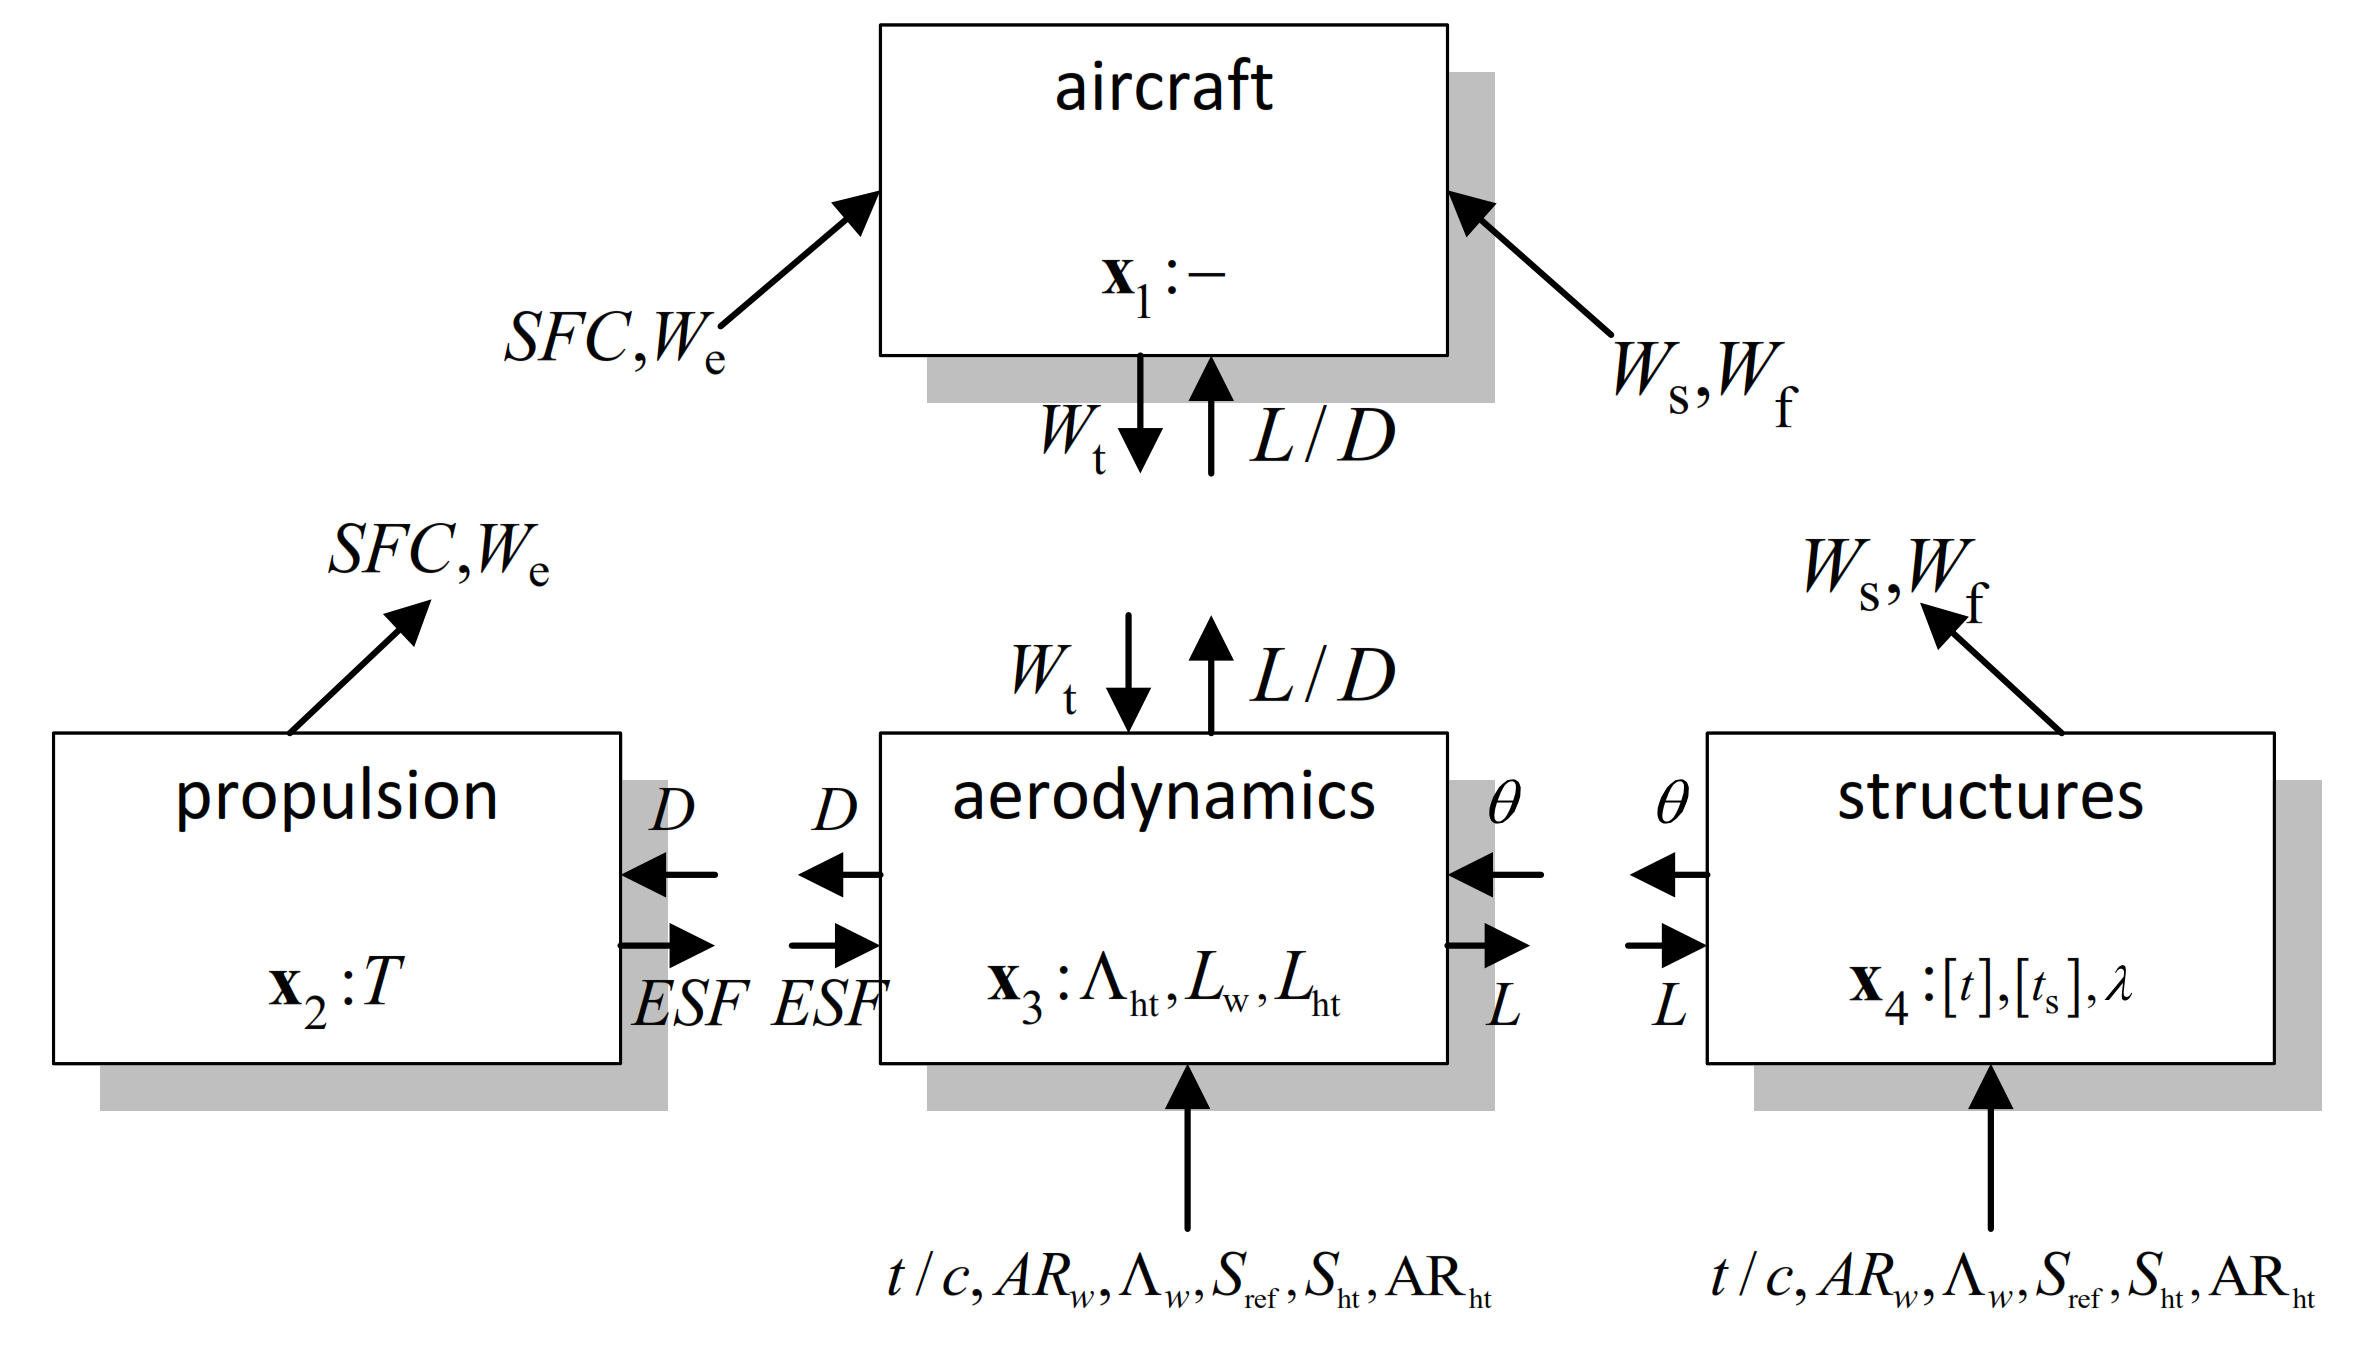
\includegraphics[height=5cm]{images/SBJ_schematics_004.png}
        \end{figure}\strut
    \end{minipage}\tabularnewline
    \begin{minipage}[t]{0.97\columnwidth}\centering
        Fig.4 Breakdown of NHATC formulation of SBJ distributed MDO
problem\strut
    \end{minipage}\tabularnewline
    \bottomrule
\end{longtable}

We can now define the properties of each variable in the table below and
code this in \url{SBJ_problem_B.py}. Again Figure 4 will help us for
bookkeeping of the distributed MDO problem's variables.

\begin{longtable}[]{@{}llllllll@{}}
\toprule
index & subproblem & name & coupling type & link & lower bound & upper
bound & baseline\tabularnewline
\midrule
\endhead
1 & 1 & \texttt{SFC} & feedback & 2 & 1 & 4 & 1.0\tabularnewline
2 & 1 & \texttt{We} & feedback & 2 & 100 & 30000 & 1.0\tabularnewline
3 & 1 & \texttt{Wt} & feedforward & 3 & 5000 & 100000 &
1.0\tabularnewline
4 & 1 & \texttt{LD} & feedback & 3 & 0.1 & 10 & 1.0\tabularnewline
5 & 1 & \texttt{Ws} & feedback & 4 & 5000 & 100000 & 1.0\tabularnewline
6 & 1 & \texttt{Wf} & feedback & 4 & 5000 & 100000 & 1.0\tabularnewline
7 & 2 & \texttt{SFC} & feedforward & 1 & 1 & 4 & 1.0\tabularnewline
8 & 2 & \texttt{We} & feedforward & 1 & 100 & 30000 & 1.0\tabularnewline
9 & 2 & \texttt{D} & feedback & 3 & 1000 & 70000 & 1.0\tabularnewline
10 & 2 & \texttt{ESF} & feedforward & 3 & 0.5 & 1.5 & 1.0\tabularnewline
11 & 2 & \texttt{T} & uncoupled & None & 0.1 & 1.0 & 1.0\tabularnewline
12 & 3 & \texttt{D} & feedforward & 2 & 1000 & 70000 &
1.0\tabularnewline
13 & 3 & \texttt{ESF} & feedback & 2 & 0.5 & 1.5 & 1.0\tabularnewline
14 & 3 & \texttt{Wt} & feedback & 1 & 5000 & 100000 & 1.0\tabularnewline
15 & 3 & \texttt{LD} & feedforward & 1 & 0.1 & 10 & 1.0\tabularnewline
16 & 3 & \texttt{theta} & feedback & 4 & 0.2 & 50 & 1.0\tabularnewline
17 & 3 & \texttt{L} & feedforward & 4 & 5000 & 100000 &
1.0\tabularnewline
18 & 3 & \texttt{tc} & shared & 4 & 0.01 & 0.1 & 1.0\tabularnewline
19 & 3 & \texttt{ARw} & shared & 4 & 2.5 & 8.0 & 1.0\tabularnewline
20 & 3 & \texttt{LAMBDAw} & shared & 4 & 40. & 70. & 1.0\tabularnewline
21 & 3 & \texttt{Sref} & shared & 4 & 200. & 800. & 1.0\tabularnewline
22 & 3 & \texttt{Sht} & shared & 4 & 50 & 148.9 & 1.0\tabularnewline
23 & 3 & \texttt{ARht} & shared & 4 & 2.5 & 8.5 & 1.0\tabularnewline
24 & 3 & \texttt{LAMBDAht} & uncoupled & None & 40. & 70. &
1.0\tabularnewline
25 & 3 & \texttt{Lw} & uncoupled & None & 0.01 & 0.2 &
1.0\tabularnewline
26 & 3 & \texttt{Lht} & uncoupled & None & 1 & 3.5 & 1.0\tabularnewline
27 & 4 & \texttt{theta} & feedforward & 3 & 0.2 & 50 &
1.0\tabularnewline
28 & 4 & \texttt{L} & feedback & 3 & 5000 & 100000 & 1.0\tabularnewline
29 & 4 & \texttt{Ws} & feedforward & 1 & 5000 & 100000 &
1.0\tabularnewline
30 & 4 & \texttt{Wf} & feedforward & 1 & 5000 & 100000 &
1.0\tabularnewline
31 & 4 & \texttt{tc} & shared & 3 & 0.01 & 0.1 & 1.0\tabularnewline
32 & 4 & \texttt{ARw} & shared & 3 & 2.5 & 8.0 & 1.0\tabularnewline
33 & 4 & \texttt{LAMBDAw} & shared & 3 & 40. & 70. & 1.0\tabularnewline
34 & 4 & \texttt{Sref} & shared & 3 & 200. & 800. & 1.0\tabularnewline
35 & 4 & \texttt{Sht} & shared & 3 & 50 & 148.9 & 1.0\tabularnewline
36 & 4 & \texttt{ARht} & shared & 3 & 2.5 & 8.5 & 1.0\tabularnewline
37 & 4 & \texttt{lambda} & uncoupled & None & 0.1 & 0.4 &
1.0\tabularnewline
38 & 4 & \texttt{t} & uncoupled & None & 0.1 & 4.0 & 1.0\tabularnewline
39 & 4 & \texttt{t} & uncoupled & None & 0.1 & 4.0 & 1.0\tabularnewline
40 & 4 & \texttt{t} & uncoupled & None & 0.1 & 4.0 & 1.0\tabularnewline
41 & 4 & \texttt{t} & uncoupled & None & 0.1 & 4.0 & 1.0\tabularnewline
42 & 4 & \texttt{t} & uncoupled & None & 0.1 & 4.0 & 1.0\tabularnewline
43 & 4 & \texttt{t} & uncoupled & None & 0.1 & 4.0 & 1.0\tabularnewline
44 & 4 & \texttt{t} & uncoupled & None & 0.1 & 4.0 & 1.0\tabularnewline
45 & 4 & \texttt{t} & uncoupled & None & 0.1 & 4.0 & 1.0\tabularnewline
46 & 4 & \texttt{t} & uncoupled & None & 0.1 & 4.0 & 1.0\tabularnewline
47 & 4 & \texttt{ts} & uncoupled & None & 0.1 & 9.0 & 1.0\tabularnewline
48 & 4 & \texttt{ts} & uncoupled & None & 0.1 & 9.0 & 1.0\tabularnewline
49 & 4 & \texttt{ts} & uncoupled & None & 0.1 & 9.0 & 1.0\tabularnewline
50 & 4 & \texttt{ts} & uncoupled & None & 0.1 & 9.0 & 1.0\tabularnewline
51 & 4 & \texttt{ts} & uncoupled & None & 0.1 & 9.0 & 1.0\tabularnewline
52 & 4 & \texttt{ts} & uncoupled & None & 0.1 & 9.0 & 1.0\tabularnewline
53 & 4 & \texttt{ts} & uncoupled & None & 0.1 & 9.0 & 1.0\tabularnewline
54 & 4 & \texttt{ts} & uncoupled & None & 0.1 & 9.0 & 1.0\tabularnewline
55 & 4 & \texttt{ts} & uncoupled & None & 0.1 & 9.0 & 1.0\tabularnewline
\bottomrule
\end{longtable}

You can follow the remaining steps in the \texttt{SBJ} method of
\url{SBJ_problem_B.py} to fully define all the inputs and outputs needed
by \texttt{DMDO} to solve the problem.

    \begin{tcolorbox}[breakable, size=fbox, boxrule=1pt, pad at break*=1mm,colback=cellbackground, colframe=cellborder]
\prompt{In}{incolor}{4}{\boxspacing}
\begin{Verbatim}[commandchars=\\\{\}]
\PY{k+kn}{from} \PY{n+nn}{SBJ\PYZus{}problem\PYZus{}B} \PY{k+kn}{import} \PY{n}{SBJ}

\PY{n}{MDAO} \PY{o}{=} \PY{n}{SBJ}\PY{p}{(}\PY{p}{)}
\PY{n}{MDAO}\PY{o}{.}\PY{n}{noprogress\PYZus{}stop} \PY{o}{=} \PY{l+m+mi}{5}
\PY{n}{out} \PY{o}{=} \PY{n}{MDAO}\PY{o}{.}\PY{n}{run}\PY{p}{(}\PY{p}{)}
\PY{n+nb}{print}\PY{p}{(}\PY{n}{out}\PY{p}{)}
\end{Verbatim}
\end{tcolorbox}

    \begin{Verbatim}[commandchars=\\\{\}]
c:\textbackslash{}Users\textbackslash{}Khalil\textbackslash{}Desktop\textbackslash{}Documents\textbackslash{}MECH\_559\_material\textbackslash{}MECH559\_notebooks\textbackslash{}10\_mdo\textbackslash{}SBJ
\_problem\_B.py:82: RuntimeWarning: invalid value encountered in double\_scalars
  g2=(2*(-outputs["CLo2"]))-(outputs["CLo1"])
c:\textbackslash{}Users\textbackslash{}Khalil\textbackslash{}Desktop\textbackslash{}Documents\textbackslash{}MECH\_559\_material\textbackslash{}MECH559\_notebooks\textbackslash{}10\_mdo\textbackslash{}SBJ
\_problem\_B.py:243: RuntimeWarning: divide by zero encountered in divide
  G1[45:48]=t1/(ts1-.1*t1)-1
c:\textbackslash{}Users\textbackslash{}Khalil\textbackslash{}Desktop\textbackslash{}Documents\textbackslash{}MECH\_559\_material\textbackslash{}MECH559\_notebooks\textbackslash{}10\_mdo\textbackslash{}SBJ
\_problem\_B.py:245: RuntimeWarning: divide by zero encountered in divide
  G1[51:54]=t3/(ts3-.1*t3)-1
c:\textbackslash{}Users\textbackslash{}Khalil\textbackslash{}Desktop\textbackslash{}Documents\textbackslash{}MECH\_559\_material\textbackslash{}MECH559\_notebooks\textbackslash{}10\_mdo\textbackslash{}SBJ
\_problem\_B.py:244: RuntimeWarning: divide by zero encountered in divide
  G1[48:51]=t2/(ts2-.1*t2)-1
    \end{Verbatim}

    \begin{Verbatim}[commandchars=\\\{\}]
0 || qmax: 0.1 || Obj: 10100.0 || dx: 51364.70503566107 || max(w): 1.0
Highest inconsistency : ESF\_3 to ESF\_2
1 || qmax: 0.050176801659138355 || Obj: 10100.0 || dx: 64286.27372124231 ||
max(w): 1.6900000000000002
Highest inconsistency : LD\_3 to LD\_1
2 || qmax: 0.05058899286830934 || Obj: 10100.0 || dx: 64646.109096676635 ||
max(w): 2.8561000000000005
Highest inconsistency : ESF\_3 to ESF\_2
3 || qmax: 0.09999999999999999 || Obj: 10100.0 || dx: 61501.778643165104 ||
max(w): 4.826809000000002
Highest inconsistency : ESF\_3 to ESF\_2
4 || qmax: 0.09999999999999999 || Obj: 10100.0 || dx: 60950.195896318386 ||
max(w): 8.157307210000004
Highest inconsistency : ESF\_3 to ESF\_2
5 || qmax: 0.07333333333333333 || Obj: 10100.0 || dx: 61823.603800931014 ||
max(w): 13.785849184900009
Highest inconsistency : LAMBDAw\_4 to LAMBDAw\_3
6 || qmax: 0.1 || Obj: 10100.0 || dx: 62783.51942832623 || max(w):
23.298085122481016
Highest inconsistency : LAMBDAw\_4 to LAMBDAw\_3
7 || qmax: 0.09999999999999999 || Obj: 10100.0 || dx: 61916.91055859945 ||
max(w): 39.37376385699292
Highest inconsistency : ARw\_4 to ARw\_3
8 || qmax: 0.09999999999999999 || Obj: 10100.0 || dx: 61184.262009307175 ||
max(w): 66.54166091831804
Highest inconsistency : ESF\_3 to ESF\_2
9 || qmax: 0.09999999999999999 || Obj: 10100.0 || dx: 61772.007012619004 ||
max(w): 112.4554069519575
Highest inconsistency : ESF\_3 to ESF\_2
10 || qmax: 0.09999999999999999 || Obj: 10100.0 || dx: 61686.550971909215 ||
max(w): 190.04963774880818
Highest inconsistency : ARw\_4 to ARw\_3
Stop: no progress after 5 iterations.
[-0.00282766 -0.02046875  0.00138316  0.00473984 -0.01526215 -0.05264995
 -0.00056961 -0.02751113  0.00040161  0.00396421 -0.1         0.01818182
  0.         -0.0085      0.          0.        ]
    \end{Verbatim}

    Let us print all the optimization variables

    \begin{tcolorbox}[breakable, size=fbox, boxrule=1pt, pad at break*=1mm,colback=cellbackground, colframe=cellborder]
\prompt{In}{incolor}{5}{\boxspacing}
\begin{Verbatim}[commandchars=\\\{\}]
\PY{k+kn}{import} \PY{n+nn}{numpy} \PY{k}{as} \PY{n+nn}{np}
\PY{n+nb}{print}\PY{p}{(}\PY{l+s+sa}{f}\PY{l+s+s1}{\PYZsq{}}\PY{l+s+s1}{\PYZhy{}\PYZhy{}\PYZhy{}\PYZhy{}\PYZhy{}\PYZhy{}Run\PYZus{}Summary\PYZhy{}\PYZhy{}\PYZhy{}\PYZhy{}\PYZhy{}\PYZhy{}}\PY{l+s+s1}{\PYZsq{}}\PY{p}{)}
\PY{n+nb}{print}\PY{p}{(}\PY{n}{MDAO}\PY{o}{.}\PY{n}{stop}\PY{p}{)}
\PY{n+nb}{print}\PY{p}{(}\PY{l+s+sa}{f}\PY{l+s+s1}{\PYZsq{}}\PY{l+s+s1}{q = }\PY{l+s+si}{\PYZob{}}\PY{n}{MDAO}\PY{o}{.}\PY{n}{Coordinator}\PY{o}{.}\PY{n}{q}\PY{l+s+si}{\PYZcb{}}\PY{l+s+s1}{\PYZsq{}}\PY{p}{)}
\PY{n}{index} \PY{o}{=} \PY{n}{np}\PY{o}{.}\PY{n}{argmax}\PY{p}{(}\PY{n}{MDAO}\PY{o}{.}\PY{n}{Coordinator}\PY{o}{.}\PY{n}{q}\PY{p}{)}
\PY{k}{for} \PY{n}{i} \PY{o+ow}{in} \PY{n}{MDAO}\PY{o}{.}\PY{n}{Coordinator}\PY{o}{.}\PY{n}{master\PYZus{}vars}\PY{p}{:}
    \PY{n+nb}{print}\PY{p}{(}\PY{l+s+sa}{f}\PY{l+s+s1}{\PYZsq{}}\PY{l+s+si}{\PYZob{}}\PY{n}{i}\PY{o}{.}\PY{n}{name}\PY{l+s+si}{\PYZcb{}}\PY{l+s+s1}{\PYZus{}}\PY{l+s+si}{\PYZob{}}\PY{n}{i}\PY{o}{.}\PY{n}{sp\PYZus{}index}\PY{l+s+si}{\PYZcb{}}\PY{l+s+s1}{ = }\PY{l+s+si}{\PYZob{}}\PY{n}{i}\PY{o}{.}\PY{n}{value}\PY{l+s+si}{\PYZcb{}}\PY{l+s+s1}{\PYZsq{}}\PY{p}{)}
\end{Verbatim}
\end{tcolorbox}

    \begin{Verbatim}[commandchars=\\\{\}]
------Run\_Summary------
No progress after several iterations
q = [-0.00282766 -0.02046875  0.00138316  0.00473984 -0.01526215 -0.05264995
 -0.00056961 -0.02751113  0.00040161  0.00396421 -0.1         0.01818182
  0.         -0.0085      0.          0.        ]
SFC\_1 = 1.0
We\_1 = 100.0
Wt\_1 = 10100.0
LD\_1 = 3.647642567519961
Ws\_1 = 5000.0
Wf\_1 = 5000.0
SFC\_2 = 1.0848297375304163
We\_2 = 6220.157215097515
D\_2 = 2344.0
ESF\_2 = 0.7248886689757545
T\_2 = 0.1
D\_3 = 2737.0329527039003
ESF\_3 = 1.0
Wt\_3 = 8786.0
LD\_3 = 3.1783982973568063
theta\_3 = 0.2
L\_3 = 8786.0
tc\_3 = 0.01
ARw\_3 = 3.5
LAMBDAw\_3 = 40.0
Sref\_3 = 661.0
Sht\_3 = 148.9
ARht\_3 = 2.5
LAMBDAht\_3 = 70.0
Lw\_3 = 0.01
Lht\_3 = 3.5
theta\_4 = 0.0
L\_4 = 5020.0
Ws\_4 = 19499.04148094153
Wf\_4 = 55017.45146845605
tc\_4 = 0.1
ARw\_4 = 2.5
LAMBDAw\_4 = 40.0
Sref\_4 = 712.0
Sht\_4 = 148.9
ARht\_4 = 2.5
lambda\_4 = 0.1
t\_4 = 4.0
t\_4 = 1.0
t\_4 = 0.1
t\_4 = 0.1
t\_4 = 4.0
t\_4 = 4.0
t\_4 = 4.0
t\_4 = 0.1
t\_4 = 0.1
ts\_4 = 0.1
ts\_4 = 2.0
ts\_4 = 1.0
ts\_4 = 1.0
ts\_4 = 9.0
ts\_4 = 9.0
ts\_4 = 0.1
ts\_4 = 9.0
ts\_4 = 9.0
range\_1 = 1999.9999368037709
Temp\_E\_2 = 1.1019125000000003
Throttle\_uA\_2 = 3176.2401155565603
Pg\_3 = 0.95
CLo1\_3 = 0.05099879167569897
CLo2\_3 = -0.00064684258462318
    \end{Verbatim}

    and print the objective \texttt{fmin} and constraint violation
\texttt{hmin}

    \begin{tcolorbox}[breakable, size=fbox, boxrule=1pt, pad at break*=1mm,colback=cellbackground, colframe=cellborder]
\prompt{In}{incolor}{6}{\boxspacing}
\begin{Verbatim}[commandchars=\\\{\}]
\PY{n}{fmin} \PY{o}{=} \PY{l+m+mi}{0}
\PY{n}{hmax} \PY{o}{=} \PY{o}{\PYZhy{}}\PY{n}{np}\PY{o}{.}\PY{n}{inf}
\PY{k}{for} \PY{n}{j} \PY{o+ow}{in} \PY{n+nb}{range}\PY{p}{(}\PY{n+nb}{len}\PY{p}{(}\PY{n}{MDAO}\PY{o}{.}\PY{n}{subProblems}\PY{p}{)}\PY{p}{)}\PY{p}{:}

    \PY{n}{fmin} \PY{o}{=} \PY{n}{MDAO}\PY{o}{.}\PY{n}{subProblems}\PY{p}{[}\PY{n}{j}\PY{p}{]}\PY{o}{.}\PY{n}{MDA\PYZus{}process}\PY{o}{.}\PY{n}{getOutputs}\PY{p}{(}\PY{p}{)}
    \PY{n}{hmin} \PY{o}{=} \PY{n}{MDAO}\PY{o}{.}\PY{n}{subProblems}\PY{p}{[}\PY{n}{j}\PY{p}{]}\PY{o}{.}\PY{n}{opt}\PY{p}{(}\PY{p}{[}\PY{n}{s}\PY{o}{.}\PY{n}{value} \PY{k}{for} \PY{n}{s} \PY{o+ow}{in} \PY{n}{MDAO}\PY{o}{.}\PY{n}{subProblems}\PY{p}{[}\PY{n}{j}\PY{p}{]}\PY{o}{.}\PY{n}{get\PYZus{}design\PYZus{}vars}\PY{p}{(}\PY{p}{)}\PY{p}{]} \PY{p}{,} \PY{n}{MDAO}\PY{o}{.}\PY{n}{subProblems}\PY{p}{[}\PY{n}{j}\PY{p}{]}\PY{o}{.}\PY{n}{MDA\PYZus{}process}\PY{o}{.}\PY{n}{getOutputs}\PY{p}{(}\PY{p}{)}\PY{p}{)}\PY{p}{[}\PY{l+m+mi}{1}\PY{p}{]}

    \PY{n+nb}{print}\PY{p}{(}\PY{l+s+sa}{f}\PY{l+s+s1}{\PYZsq{}}\PY{l+s+s1}{SP\PYZus{}}\PY{l+s+si}{\PYZob{}}\PY{n}{MDAO}\PY{o}{.}\PY{n}{subProblems}\PY{p}{[}\PY{n}{j}\PY{p}{]}\PY{o}{.}\PY{n}{index}\PY{l+s+si}{\PYZcb{}}\PY{l+s+s1}{: fmin= }\PY{l+s+si}{\PYZob{}}\PY{n}{fmin}\PY{l+s+si}{\PYZcb{}}\PY{l+s+s1}{), hmin= }\PY{l+s+si}{\PYZob{}}\PY{n}{hmin}\PY{l+s+si}{\PYZcb{}}\PY{l+s+s1}{\PYZsq{}}\PY{p}{)}
    \PY{k}{if} \PY{n}{MDAO}\PY{o}{.}\PY{n}{subProblems}\PY{p}{[}\PY{n}{j}\PY{p}{]}\PY{o}{.}\PY{n}{is\PYZus{}main}\PY{p}{:}
        \PY{n}{fmin} \PY{o}{=} \PY{n}{MDAO}\PY{o}{.}\PY{n}{subProblems}\PY{p}{[}\PY{n}{j}\PY{p}{]}\PY{o}{.}\PY{n}{MDA\PYZus{}process}\PY{o}{.}\PY{n}{getOutputs}\PY{p}{(}\PY{p}{)}
        \PY{n}{hmin} \PY{o}{=} \PY{n}{MDAO}\PY{o}{.}\PY{n}{subProblems}\PY{p}{[}\PY{n}{j}\PY{p}{]}\PY{o}{.}\PY{n}{opt}\PY{p}{(}\PY{p}{[}\PY{n}{s}\PY{o}{.}\PY{n}{value} \PY{k}{for} \PY{n}{s} \PY{o+ow}{in} \PY{n}{MDAO}\PY{o}{.}\PY{n}{subProblems}\PY{p}{[}\PY{n}{j}\PY{p}{]}\PY{o}{.}\PY{n}{get\PYZus{}design\PYZus{}vars}\PY{p}{(}\PY{p}{)}\PY{p}{]} \PY{p}{,} \PY{n}{MDAO}\PY{o}{.}\PY{n}{subProblems}\PY{p}{[}\PY{n}{j}\PY{p}{]}\PY{o}{.}\PY{n}{MDA\PYZus{}process}\PY{o}{.}\PY{n}{getOutputs}\PY{p}{(}\PY{p}{)}\PY{p}{)}\PY{p}{[}\PY{l+m+mi}{1}\PY{p}{]}
        \PY{k}{if} \PY{n+nb}{max}\PY{p}{(}\PY{n}{hmin}\PY{p}{)} \PY{o}{\PYZgt{}} \PY{n}{hmax}\PY{p}{:}
            \PY{n}{hmax} \PY{o}{=} \PY{n+nb}{max}\PY{p}{(}\PY{n}{hmin}\PY{p}{)}
\PY{n+nb}{print}\PY{p}{(}\PY{l+s+sa}{f}\PY{l+s+s1}{\PYZsq{}}\PY{l+s+s1}{P\PYZus{}main: fmin= }\PY{l+s+si}{\PYZob{}}\PY{n}{fmin}\PY{l+s+si}{\PYZcb{}}\PY{l+s+s1}{, hmax= }\PY{l+s+si}{\PYZob{}}\PY{n}{hmax}\PY{l+s+si}{\PYZcb{}}\PY{l+s+s1}{\PYZsq{}}\PY{p}{)}
\PY{n+nb}{print}\PY{p}{(}\PY{l+s+sa}{f}\PY{l+s+s1}{\PYZsq{}}\PY{l+s+s1}{Final obj value of the main problem: }\PY{l+s+se}{\PYZbs{}n}\PY{l+s+s1}{ }\PY{l+s+si}{\PYZob{}}\PY{n}{fmin}\PY{l+s+si}{\PYZcb{}}\PY{l+s+s1}{\PYZsq{}}\PY{p}{)}
\end{Verbatim}
\end{tcolorbox}

    \begin{Verbatim}[commandchars=\\\{\}]
SP\_1: fmin= [10100.0, 1999.9999368037709]), hmin= [3.1598114569320046e-08]
SP\_2: fmin= [1.0848297375304163, 6220.157215097515, 0.7248886689757545,
1.1019125000000003, 3176.2401155565603]), hmin= [0.08030637254901984,
-0.49097047415236283]
SP\_3: fmin= [8786.0, 2737.0329527039003, 3.1783982973568063, 0.95,
0.05099879167569897, -0.00064684258462318]), hmin= [-0.13636363636363646,
-0.05229247684494533, -0.04970510650645261]
SP\_4: fmin= [19499.04148094153, 55017.45146845605, 0.0]), hmin=
[-0.8763362226531818, -0.9972602790723825, -0.9965166338503441,
-0.9903729029499353, -0.9999919107125058, -0.9999952356481218,
-0.9955393323478647, -1.0000080892717282, -1.000004764351695,
-0.9986794225715389, -0.996041744430522, -0.9821633572119252,
-0.9899739919255813, -0.948639567433413, -0.6487218959747043,
-1.0100122409310999, -1.0507817968089146, -1.235655927546862,
-0.8769331440834405, -0.9972709378660298, -0.996518688072637,
-0.9904407419168215, -0.9999919107125818, -0.9999952356481226,
-0.9956071713147511, -1.0000080892718042, -1.0000047643516958,
-0.7877406196875452, -0.9896049001468968, -0.9961238006559385,
-0.9986794225715389, -0.9633321585432101, -0.9821633572119252,
-1.0100122409310999, -1.1202313729661217, -1.014611691842359,
-0.9899739919255813, -0.8685955310376006, -0.9850959123979508,
-0.9655250777658886, -0.9904765123299427, -0.9967191883899331,
-0.9969732157051322, -0.6892103057634813, -0.3943318251002417,
-14.333333333333332, -0.4736842105263158, -0.898989898989899,
-0.898989898989899, -0.5348837209302326, -0.5348837209302326,
-14.333333333333332, -0.9888765294771968, -0.9888765294771968,
-1.1236637773468183, -1.0027397209276177, -1.003483366149656,
-1.001320577428461, -1.003958255569478, -1.0178366427880747,
-1.1230668559165595, -1.0027290621339702, -1.003481311927363,
-1.2122593803124548, -1.0103950998531033, -1.0038761993440615,
-1.001320577428461, -1.03666784145679, -1.0178366427880747, -1.0344749222341114,
-1.0095234876700574, -1.0032808116100669]
P\_main: fmin= [19499.04148094153, 55017.45146845605, 0.0], hmax=
3.1598114569320046e-08
Final obj value of the main problem:
 [19499.04148094153, 55017.45146845605, 0.0]
    \end{Verbatim}


    % Add a bibliography block to the postdoc
    
    
    
\end{document}
